\documentclass[12pt]{article}
\usepackage[utf8]{inputenc}
\usepackage[letterpaper, margin=.75in]{geometry}
\usepackage{graphicx}
\usepackage{mathptmx}
\usepackage{float}
\usepackage[cmex10]{amsmath}
\usepackage{amsthm,amssymb}
\usepackage{url}
\urlstyle{same} 
\def\UrlBreaks{\do\/\do-}
\usepackage{breakurl}
\usepackage{fancybox}
\usepackage{breqn}
\usepackage{array}
\usepackage{caption}
\usepackage{subcaption}
\usepackage{comment}
\usepackage[english]{babel}
\usepackage[acronym,nomain]{glossaries} % list of acronyms
\usepackage{xurl}
\usepackage{multicol}
\usepackage{multirow}
\usepackage{mathptmx}
\usepackage{float}
\usepackage{lipsum}
\usepackage{framed}
\usepackage{empheq}
\usepackage[T1]{fontenc}

\renewcommand{\arraystretch}{1.2}
\newcommand{\figurewidth}{.67\linewidth}

\sloppy

\newcolumntype{C}[1]{>{\centering\let\newline\\\arraybackslash\hspace{0pt}}m{#1-2\tabcolsep}}

\setlength{\columnsep}{.25in}

\usepackage[%
backend=bibtex,     % biber or bibtex
%style=authoryear,    % Alphabeticalsch
style=numeric-comp , % numerical-compressed
sorting=none,        % no sorting
sortcites=true,      % some other example options ...
block=none,
indexing=false,
citereset=none,
isbn=true,
url=true,
doi=true,            % prints doi
natbib=true,         % if you need natbib functions
]{biblatex}
\addbibresource{./sources/sources}  % better than \bibliography

\usepackage[
pdfpagelabels,
pdfusetitle,
hidelinks,
colorlinks = true,
linkcolor = blue,
citecolor = blue,
pdfborder = {0 0 0}
]{hyperref}

\title{Designing Better Charging Networks: Charging Network Expansion Optimization Accounting for Queuing Dynamics}
\author{Aaron Rabinowitz \textit{et al.}}
\date{}

\newacronym{good}{GOOD}{Grid Optimized Operation Dispatch}
\newacronym{od}{OD}{Economic Dispatch}
\newacronym{ce}{CE}{Capacity Exapnsion}
\newacronym{soc}{SOC}{State of Charge}
\newacronym{mud}{MUD}{Multi-Unit Dwelling}
\newacronym{bev}{BEV}{Battery Electric Vehicle}
\newacronym{ess}{ESS}{Energy Storage System}
\newacronym{icev}{ICEV}{Internal Combustion Engine Vehicle}
\newacronym{frp}{FRP}{Flow Refueling Problem}
\newacronym{esn}{ESN}{Energy Supply Network}
\newacronym{afdc}{AFDC}{Alternative Fuels Data Center}
\makeglossaries

\begin{document}

\maketitle

%\begin{multicols}{2}

%\lipsum[55]

\section{Introduction}

%Infrastructure networks tend to evolve in three phases; connecting, balancing, and hardening. In the first phase minimum service is provided for all users. In the second phase high usage elements are upgraded to meet observed demand. In the third phase, redundant elements are added in order to accommodate overflow demand and to maintain functionality in the case of element failure. 

\gls{bev} charging infrastructure is relatively new when compared to other transportation infrastructure systems. Per \gls{afdc}, the number of public charging stations in the US increased by more than 800\% in the decade between 2013 and 2023 \cite{Brown_2023}. The number is certainly much higher when factoring in private charging stations but less is known about these \cite{Davis_2022}. Most of these stations are small AC charging stations and serve primarily to meet daily travel needs. Of the stations currently tracked by \gls{afdc}, about 16.5\% are DC charging stations which must, by necessity, serve as the backbone of long distance \gls{bev} travel.

The current charging network in the US is spatially unequal. In some areas of the country the DC charging network is quite sparse and, in others, quite dense. There are only 66 total DC stations in the state of Idaho with a total of 193 ports between them. The vast majority of these are on Interstate highways between the large population centers of Boise and Idaho Falls. By contrast, California contains nearly 2,500 DC stations with over 14,000 ports. These networks are, plainly, in different phases of their development.

The purpose of a travel infrastructure network is to induce travel by reducing its cost. Different users will evaluate cost differently \citep{Ortuzar_2024, Raveau_2016, BenAkiva_2004} and, oftentimes, the difference in costs between multiple routes will fall within an individual's threshold of disambiguation, especially if costs are uncertain \cite{DePalma_2005}. In general, travelers are sensitive to prices and travel times \cite{Hongli_2017} both of which are results of network design. Travel-mode specific characteristics matter in optimizing design. \glspl{bev} and \glspl{icev} share the same roads but draw energy from entirely separate networks. This means that for sufficiently long trips, they should be considered as different travel modes. At a typical US fueling rate of 7 gallons per minute, a gasoline powered vehicle is adding energy at a rate of 14.15 MW. High-end \glspl{bev} charge at maximum rates of around 350 kW. \glspl{bev} are 3-5 times more efficient \citep{ev_database_2025} but the effect is that \gls{bev} charging events are substantially longer than \glspl{icev} fueling events. DC chargers are, also, more expensive to install than liquid fuel pumps \cite{Miller_2024, Nicholas_2019} with the cost depending on a number of factors including the cost of upgrading the power grid to support the station \cite{Gamage_2023}. The cost differential meas that fueling station operators can add capacity to meet demand far easier than charging station operators can. As a result, fueling station congestion is not usually an issue but charging station congestion is an emerging adoption bottleneck \citep{Jenn_2025}.

The performance of an \gls{esn} (charging/fueling network) is the travel-time tax imposed on users by the structure of the network. The travel-time tax is the amount of travel-time added due to the need to charge/fuel. A better designed \gls{esn} imposes a smaller tax. \gls{esn} structure increases travel-time in three ways: 1) time required to detour from the shortest route to use a station, 2) time spent queuing at the station before the charging/fueling event, and 3) time spent during the charging/fueling event.

The literature on optimal charging/fueling network expansion is dominated by methodology well suited to fueling network design. In this paradigm stations are a fungible unit. The most significant time penalty is due to detouring. Thus, the decision of where to locate stations is the most important determinant of network performance. Once in place, a station may be designed to store and dispense fuel as needed. For charging networks, a different paradigm is needed. Because charging events are long, queues are likely to form. The number of chargers, power dispensing capability of the chargers, and physical layout of the station impact how efficiently the queue will clear, and thus the actual capacity of the station, in nonlinear but predictable ways. Adding a given number of stations or chargers can lead to very different performance gains depending on the manner in which they are allocated.

This paper presents a novel method for charging network optimal expansion accounting for all elements of travel-time tax. This method is an improvement over previous methodology for planning the expansion of charging networks, particularly those which are in the balancing phase of development. Specific contributions of this paper are:

\begin{enumerate}
	\item A novel formulation for the optimal \gls{esn} expansion problem accounting for expected queuing delay at stations. The optimization code is provided as a Python package.
	\item An application of said formulation to a real-life case study with generalizable takeaways.
\end{enumerate}


%In the connecting phase, it is sufficient to ask where should stations be located such that all origin-destination pairs are connected. Where the DC charging network has guaranteed connectivity, the next priority is balancing demand and supply. It is pertinent to note that the amount of "supply" a network provides is not captured by a single number such as total stations or total chargers. The composition of a network in terms of locations, speeds, and port counts of stations matter but cannot be evaluated independent of demand. Much research has been performed in the field of charging network capacity expansion optimization. The vast majority of this research is connectivity-oriented and ignores the effects of station composition.
\section{Literature Review}

The the problem of optimal \gls{esn} expansion belongs to the larger field of strategic facility location optimization, a fundamental problem in operations research \citep{Owen_1998}. The optimal \gls{esn} expansion problem seeks to find the set of station locations and characteristics which most efficiently serves a set of demands. The literature on the optimal \gls{esn} expansion problem can be categorized by scope and approach.

\subsection{Scope}

\subsubsection{Demand}

Considered from a system-level perspective, the underlying goal of the optimization is multi-objective: to find a solution which minimizes user costs and infrastructure costs. The optimal \gls{esn} expansion problem must begin with a definition of demand, user costs, and infrastructure costs.

Demand may be defined by locations (nodal), or trips/tours (travel) \citep{Metais_2022_rser}. Nodal demand formulations attempt to minimize the cost of relocating from locations where users will be when they desire to charge to charging locations. This is accomplished by assigning equipment to locations and demand nodes to equipment. Nodal demand studies have employed various formulations to optimize around technical, economic, and environmental objectives and constraints \citep{Zhu_2018_jssse, Yi_2019_e, Xiao_2020_jes, Ma_Xie_2021_trd, Kuby_2023_he, Faustino_2023_e, Gupta_2023_jes, Liu_2023_ijst, Weekx_2024_trr, Yuvaraj_2024_ia, Davatgari_2024_ejor, Tungom_2024_esa, Vijay_2024_es, Wu_2024_trd}. Nodal demand problems are most relevant to planning on a municipal scale. Most travel is routine and short-distance \citep{NHTS_2017, NHTS_2022}, and most charging is accomplished during long-dwells \citep{Hardman_2018}. Access to low-rate charging is an important aspect of \gls{bev} user convenience \citep{Rabinowitz_2023_ia}.

Travel demand formulations attempt to minimize the added cost of charging/fueling for itineraries which are likely to exceed vehicle range. This is accomplished by assigning equipment to locations and flows to equipment. Charging and fueling add time to trips because of the time required to charge/fuel, the time required to wait for available equipment, and the time required to deviate from one's route to reach a station. Flow-capturing formulations optimize an \gls{esn} to best serve traffic flows along the routes they normally take, often the shortest path \citep{Kuby_2005_seps, Kuby_2007_nse, Upchurch_2009_ga}. Flow-enabling formulations optimize and \gls{esn} to best enable traffic flows by dictating what routes they will take from a set of possible paths \citep{Kim_2012_ijhe, MirHassani_2013_ts, Huang_Li_2015_nse, Li_Huang_2016_trc, Zhang_2017_trb, Tian_2018_s, Arslan_2019_ts, Anjos_2020_ejor, Wu_2024_e, Zeng_2024_mt, Ala_2024_scis, Pourvaziri_2024_tre}. Travel demand problems are most relevant to regional-scale planning.

\subsubsection{User Costs}

Maximizing level-of-service is accomplished by minimizing user-costs. Failing to account for an aspect of user-cost is equivalent to assuming zero cost. User costs are composed of: 

\begin{description}
	\item[Cost-to-Travel] Cost of traveling to a station or deviating from the shortest-path to utilize a station
	\item[Cost-to-Wait] Cost of waiting to charge
	\item[Cost-to-Charge] Cost of charging
	\item[Cost-of-Failure] Cost of failing to charge at a given station.
\end{description}

Every study surveyed includes cost-to-travel. For nodal demand, the cost-to-travel scales with the distance from the origin node to the station \citep{Zhu_2018_jssse, Yi_2019_e, Xiao_2020_jes, Ma_Xie_2021_trd, Kuby_2023_he, Faustino_2023_e, Gupta_2023_jes, Liu_2023_ijst, Weekx_2024_trr, Yuvaraj_2024_ia, Davatgari_2024_ejor, Tungom_2024_esa, Vijay_2024_es, Wu_2024_trd} where each origin-station pair has a unique cost. Because it is inconvenient to have to travel a substantial distance specifically to charge \citep{Rabinowitz_2023_ia}, the felt cost of traveling may increase exponentially with distance and many stations will be effectively unreachable. For travel demand, the cost-to-travel scales with the selected alternate path's distance \citep{Kuby_2005_seps, Kuby_2007_nse, Upchurch_2009_ga, Kim_2012_ijhe, MirHassani_2013_ts, Huang_Li_2015_nse, Li_Huang_2016_trc, Zhang_2017_trb, Tian_2018_s, Arslan_2019_ts, Anjos_2020_ejor, Wu_2024_trd, Zeng_2024_mt, Ala_2024_scis, Pourvaziri_2024_tre}. As overall trip length increases, the importance of deviation paths to total trip distance decreases and, often, many paths will be close enough in cost to the shortest-path to be considered viable alternatives.

The cost-to-wait is often not modeled. Optimal \gls{esn} expansion methodology is rooted in fueling network optimization where negligible at-station waiting times may be assumed. Because \glspl{bev} have shorter ranges and are slower to charge than \glspl{icev}, waiting cannot be safely assumed to be zero. Where the cost-to-wait is accounted for, a queuing model is applied. Queuing theory provides established formulae for computing an expectation of waiting time based on the distribution of arrival times, distribution of service times, and number of servers. The parameters of these formulae are set by station demand, charging speeds, and number of chargers. The relationship between arrival rate and waiting time is nonlinear and approaches infinity as arrival rate approaches the maximum throughput of the station. Queuing models are used to represent the time cost of waiting \citep{Zhu_2018_jssse, Tian_2018_s, Yi_2019_e, Wang_2022_er, Vijay_2024_es, Pourvaziri_2024_tre} or to compute the maximum allowable arrival rate or minimum number of chargers \citep{Xiao_2020_jes, Wu_2024_trd}.

The cost-to-charge is sometimes modeled and sometimes ignored. In reality, the time required to charge an \glspl{bev} is dependent on many factors including the maximum nominal rates allowed by the charger and vehicle (each of which is effected by external conditions) and the starting and final \gls{soc} of the event. Most \glspl{bev} will feature a nearly linear phase of charging followed by phase where the charge rate declines exponentially \citep{Marra_2012}. It is possible for a path featuring two charge events which are exclusively in the linear phase to be shorter than a path featuring one event which extends into the exponential decay phase. If linear charging ranges and homogeneous charging equipment are assumed then the cost-of-charging will scale linearly with path energy consumption and can be ignored. Studies which do not account for cost-to-charge  either implicitly or explicitly use this logic. Where cost to charge is accounted for, this can be done by accounting for chargers with different maximum rates and/or accounting for different final \gls{soc} \citep{Davatgari_2024_ejor, Yuvaraj_2024_ia, Zhu_2018_jssse, Upchurch_2009_ga, Zhang_2023_ijpr, Tian_2018_s, Vijay_2024_es, Wang_2022_er, Wu_2024_trd}. The price of a charge event is usually ignored but may be accounted for if the topology of the power grid is also modeled \citep{Yuvaraj_2024_ia, Gupta_2023_jes, Vijay_2024_es, Yi_2019_e}. However, a direct and causal relationship between grid topology and charging prices at any given station is not reflective of reality as charging prices usually reflect regional electricity prices \cite{Trinko_2021}.

The cost-of-failure is either an implicit or explicit element of the optimization. For a variety of reasons, a given station or path might be infeasible for a given vehicle. If no station or path is feasible for that vehicle then then the \gls{esn} has partially failed. These failures can either be priced in (maximal-coverage) or used as a constraint (set-coverage). For set-coverage formulations, the most common form requires at least a given portion of demand to be accommodated \citep{Ala_2024_scis, Anjos_2020_ejor, Arslan_2019_ts, Davatgari_2024_ejor, Pourvaziri_2024_tre, Tian_2018_s, Wu_2024_trd, Vijay_2024_es, Xiao_2020_jes, Yi_2019_e, Zhang_2023_ijpr, Zhu_2018_jssse}. A sort of hybrid approach can be taken where the optimization is formulated as a set-coverage problem but the options (stations or paths) are limited to only those which might reasonably be taken \citep{Faustino_2023_e, Gupta_2023_jes, Huang_Li_2015_nse, Kim_2012_ijhe, Kuby_2005_seps, Kuby_2007_nse, Kuby_2023_he, Li_Huang_2016_trc, Ma_Xie_2021_trd, MirHassani_2013_ts, Tungom_2024_esa, Upchurch_2009_ga, Zhang_2017_trb}.

\subsubsection{Infrastructure Costs}

Building out the optimal \gls{esn} comes at a cost. The components of infrastructure cost are:

\begin{description}
	\item[Station-Costs] Cost of all operations required to open a station before adding chargers and independent of size and power draw.
	\item[Charger-Costs] Costs of procuring and installing chargers and associated size-scaling equipment.
	\item[Grid-Costs] Cost of upgrading the grid to deliver sufficient power to the station.
\end{description}

It is common to ignore infrastructure costs altogether or to treat stations as fungible units of which a certain amount can be deployed. Where infrastructure costs are modeled, the elements of cost are modeled in a relatively common manner. Fixed-costs can be amortized among all chargers in the station and the inclusion of fixed costs means that larger stations will be more cost efficient on a per-charger basis \citep{Ala_2024_scis, Anjos_2020_ejor, Pourvaziri_2024_tre, Vijay_2024_es, Wang_2022_er, Wu_2024_trd, Xiao_2020_jes, Zhang_2023_ijpr, Zhu_2018_jssse}. Charger-costs scale linearly with the number of chargers installed \citep{Ala_2024_scis, Anjos_2020_ejor, Davatgari_2024_ejor, Gupta_2023_jes, Pourvaziri_2024_tre, Vijay_2024_es, Wang_2022_er, Wu_2024_trd, Xiao_2020_jes, Zhang_2023_ijpr, Zhu_2018_jssse} of a given type and may include operations and maintenance \citep{Yi_2019_e, Zhu_2018_jssse}. Grid-costs may be location specific or a general model and may effect the price of electricity at a station. Grid costs may scale with chargers \cite{Yi_2019_e} or may be modeled using a representation of a distribution grid \cite{Gupta_2023_jes, Vijay_2024_es}.

In general, the cost models employed provide a fixed cost for opening a station and then other costs scale with he station size and electricity demand. As fixed costs are only applied once, this incentivizes larger stations over smaller stations all else being equal. This model of costs reflects reality as larger installations come at a lower cost-per-charger price \citep{Nicholas_2019}. Power grid upgrade costs are a substantial portion of the total cost \citep{Gamage_2023} but modeling these costs is quite inexact when dealing with distribution grids \citep{Li_2024_pnas}. The decision to include or not include the various infrastructure costs reflects scoping decisions and there is a general divide between transportation focused studies and energy focused studies reflected in the absence or presence of a grid cost component.

\subsection{Approach}

Considered from a system-level perspective, the underlying goal of the optimization is multi-objective: to find a solution which maximizes level-of-service while minimizing infrastructure cost. These objectives are inherently conflicting. The literature surveyed can be separated into exact and approximate approaches. In order to compute an exact solution, one must either define an equivalence between infrastructure cost and level-of-service or optimize for one subject to a constraint on the other. The problem can then be solved using an optimal \gls{milp} or \gls{minlp} solver. Alternatively, an approximate solution may be found using dominance methodology utilizing metaheuristics such as \gls{nsga} \citep{Deb_2002_tec} or a related algorithm. Approximate approaches are used to reveal the Pareto surface between user costs and infrastructure costs and are most useful in the conceptualization phase of a project. Exact approaches solve well defined problems and will be more useful in a project's planning stage.

Regardless of approach, most papers surveyed contained continuous and integer elements. The continuous aspects of the problem concern fractional assignment of demand elements to stations and other variables such energy dispensed and queue waiting times. The integer elements are those elements which define network structure such as the location and size of stations and grid equipment. Approximate approaches tend to feature complex and multifaceted objective functions designed to give a user a complete understanding of the trade-offs in network design. Exact approaches tend to feature simple objectives and run-time optimized methodology. Exact approaches often reduce the problem to an effort to find a set of station locations which connect all demands. This simplifying assumption can be leveraged to drastically reduce the design space and improve computational efficiency \cite{Arslan_2019_ts}.

The two approaches described represent a common trade-off in optimization. Approximate methods allow for the consideration of ever more factors and complex nonlinear behavior. This comes with the drawback of being hyper-parameter dependent. In order to utilize the full capability of these methods, one needs a tremendous amount of exact data and a tremendous amount of computational cycles. Exact methods require simpler and more straightforward formulations but bring a level of transparency and can be heavily optimized for run-time scaling.

\subsection{Summary}

Optimal \gls{esn} expansion is a well studied problem. The methodology seen in the surveyed literature approaches the optimal \gls{esn} expansion problem form a variety of perspectives. These perspectives include those of transportation planners and policy makers, \gls{esn} operators, and power system operators. The studies surveyed also reflect different levels of specificity with methods designed for high-level and extremely detailed analysis. For most of these papers, advancing the methodology is the core contribution. Case studies in optimization papers are often performed on networks that are unrealistically small in scale and with complete information.

The focus of this study is to demonstrate the effects of station composition on \gls{esn} performance for long-trip travel at a strategic/policy level. As a result, the method is deliberately limited in scope and designed to be as simple as possible while retaining the capability to answer the questions asked. The specific focus of the model dictates several decisions. First, the model focuses nearly entirely on user costs. Policy makers and strategic decision makers should be primarily concerned with improving user experience and secondarily with achieving maximum efficiency in pursuit of this goal. Further, the costs of purchasing land and upgrading the distribution power grid are difficult to predict and context dependent. These factors will, no doubt, influence decisions on a micro level but will not impact a general understanding of the relationship between \gls{esn} structure of performance. As such, user costs are modeled in detail while infrastructure costs are modeled in the simplest manner possible. Second, in pursuit of a clear and transparent model, an exact approach was selected. Although metaheuristic optimization offers the ability to efficiently explore complex design spaces, it does so at the cost of hyperparameter dependence. It is impossible for one to make an obvious case for which precise form of a metaheuristic algorithm and which precise sets of tuning parameters are the best combination for the optimal \gls{esn} expansion problem. Any paper which uses such a method must devote substantial space to explaining and justifying the method itself. By contrast, an exact approach can utilize an exiting and rigorously proven optimal solver.

The method presented models all elements of user cost accounting for additional driving time, queuing time, charging time, and the cost of failing to accommodate demand and does so in an efficient manner. A key element of this method are a linearized M/M/c queuing model. This model is then applied for a case study on a very large network where the impact of \gls{esn} structure on performance at varying demand levels is demonstrated along with the very high impact of targeted expansion. The case study provides generalizable takeaways which are of value to policy makers and strategic planners. 

%The two approaches described represent a common trade-off in optimization. Approximate methods allow for the consideration of ever more factors and complex nonlinear behavior. This comes with the drawback of being hyper-parameter dependent. In order to utilize the full capability of these methods, one needs a tremendous amount of exact data and a tremendous amount of computational cycles. Exact methods require simpler and more straightforward formulations but bring a level of transparency and can be optimized.

%Problem complexity will scale exponentially with the scale of the network being optimized. Of the papers surveyed, only \cite{Arslan_2019_ts} presented a case study on a truly large network using a minimalist method.

%An \gls{esn} must be designed to meet demand. Demand may be defined by locations (nodal), or trips/tours (travel) \citep{Metais_2022}. Nodal demand formulations attempt to minimize the cost of relocating from locations where users will be when they desire to charge to charging locations. This is accomplished by assigning equipment to locations and demand nodes to equipment. Nodal demand studies have employed various formulations \citep{Kuby_2023} to optimize around technical, economic, and environmental objectives and constraints \citep{Yuvaraj_2024, Faustino_2023, Gupta_2023}. Variations introduce stochasticity \citep{Tungom_2024, Wu_Fainman_2024}, fleet operations \citep{Davatgari_2024, Ma_Xie_2021}, nonlinear queuing \citep{Liu_2023} dynamics, and over-flow relocation \citep{Weekx_2024}. Nodal demand problems are most relevant to planning on a municipal scale. Most travel is routine and short-distance \cite{NHTS_2017, NHTS_2022}, and most charging is accomplished during long-dwells \citep{Hardman_2018}. Access to low-rate charging is an important aspect of \gls{bev} user convenience \citep{Rabinowitz_2023}.
%
%Travel demand formulations attempt to minimize the added cost of charging/fueling for itineraries which are likely to exceed vehicle range. This is accomplished by assigning equipment to locations and flows to equipment. Charging and fueling add time to trips because of the time required to charge/fuel, the time required to wait for available equipment, and the time required to deviate from one's route to reach a station. Flow-capturing formulations optimize an \gls{esn} to best serve traffic flows along the routes they normally take, often the shortest path \citep{Kuby_2005, Kuby_2007, Upchurch_2009}. Flow-enabling formulations optimize and \gls{esn} to best enable traffic flows by dictating what routes they will take from a set of possible paths \citep{Kim_2012, MirHassani_2013, Huang_Li_2015, Li_Huang_2016, Zhang_2017, Arslan_2019, Anjos_2020, Wu_2024, Zeng_2024, Ala_2024}. Travel demand problems are most relevant to regional-scale planning.










\section{Methods}

Previous work considers the function of an \gls{esn} to be to connect origins and destinations for a set of demand flows whose distance exceeds vehicle range. This approach is valid but limits the scope of analysis. The approach in this paper considers the function of an \gls{esn} as being to minimize the time-cost imposed by the need to refuel/recharge on drivers of a given vehicle type. For a set of demands defined by origin, destination, and volume, the minimum overall travel time is the overall travel time if all vehicles take their shortest path. This forms a lower bound. Any time spent deviating to a station or at the station can be thought of as a cost imposed by the structure of the \gls{esn}. If travel between an origin and destination is impossible or sufficiently difficult, the driver might pick a different mode (such as air travel) or rent a vehicle of a different fuel type. This forms an upper bound. The method presented here is an optimal \gls{esn} expansion problem which minimizes the travel cost imposed by the \gls{esn}.

\subsection{Supply Network Graphs}

Consider a road network represented by a directed graph $G_R = \{V_R, E_R\}$ where $V_R$ is a set of nodes and $E_R$ is a set of edges. The set of nodes $V_R$ contains places (cities and towns) at the nodes in $V_{P} \subseteq V_R$ and stations at the nodes in $V_{S} \subseteq V_R$. The set of edges $E_R$ contains road links. Drivers may pass by places and stations without stopping and drivers who take the same road path will not necessarily stop at the same stations. Thus, it is useful to transform the graph as in \citep{MirHassani_2013}. Transformed graph $G = \{V, E\}$ contains nodes $V = V_S \cup V_P$ and the edges in $E$ are paths taken along the road network. $E$ contains edges for all pairs in $V$ if the energy consumption required is less than the vehicle \gls{ess} capacity.  Routes along $G_R$ are road-paths. Routes along $G$ are supply-paths. It is not possible for any edge $(i, j) \in E$ to have negative cost thus only simple supply-paths need to be considered.

As is the case in prior work, the method presented requires a set of alternative paths for each origin-destination flow. These paths are found using a k-path routing algorithm \citep{Yen_1971, Qian_2013, Eppstein_1998}. In order to guarantee that the alternative paths are simple paths a second transformation is made. For every place $o \in V_P$ which serves as a demand origin, a level graph $\overline{G}_o = \{V, \overline{E}\}$ is constructed where $\overline{E} \subseteq \hat{E}$ and all edges $(i, j) \in \overline{E}$ lead away from $o$. The graph transformations are demonstrated in Figure \ref{fig:paths}



%In order to facilitate in finding the $k$ shortest simple supply-paths, for each origin $o \in V_P$, a level graph $\overline{G}_o = \{V, \overline{E}\}$ is constructed where $\overline{E} \subseteq \hat{E}$ and all edges $(i, j) \in \overline{E}$ lead away from $o$. Using $\overline{G}$ the $k$ shortest simple supply-paths are found using Yen's method.

\begin{figure}[H]
	\centering
	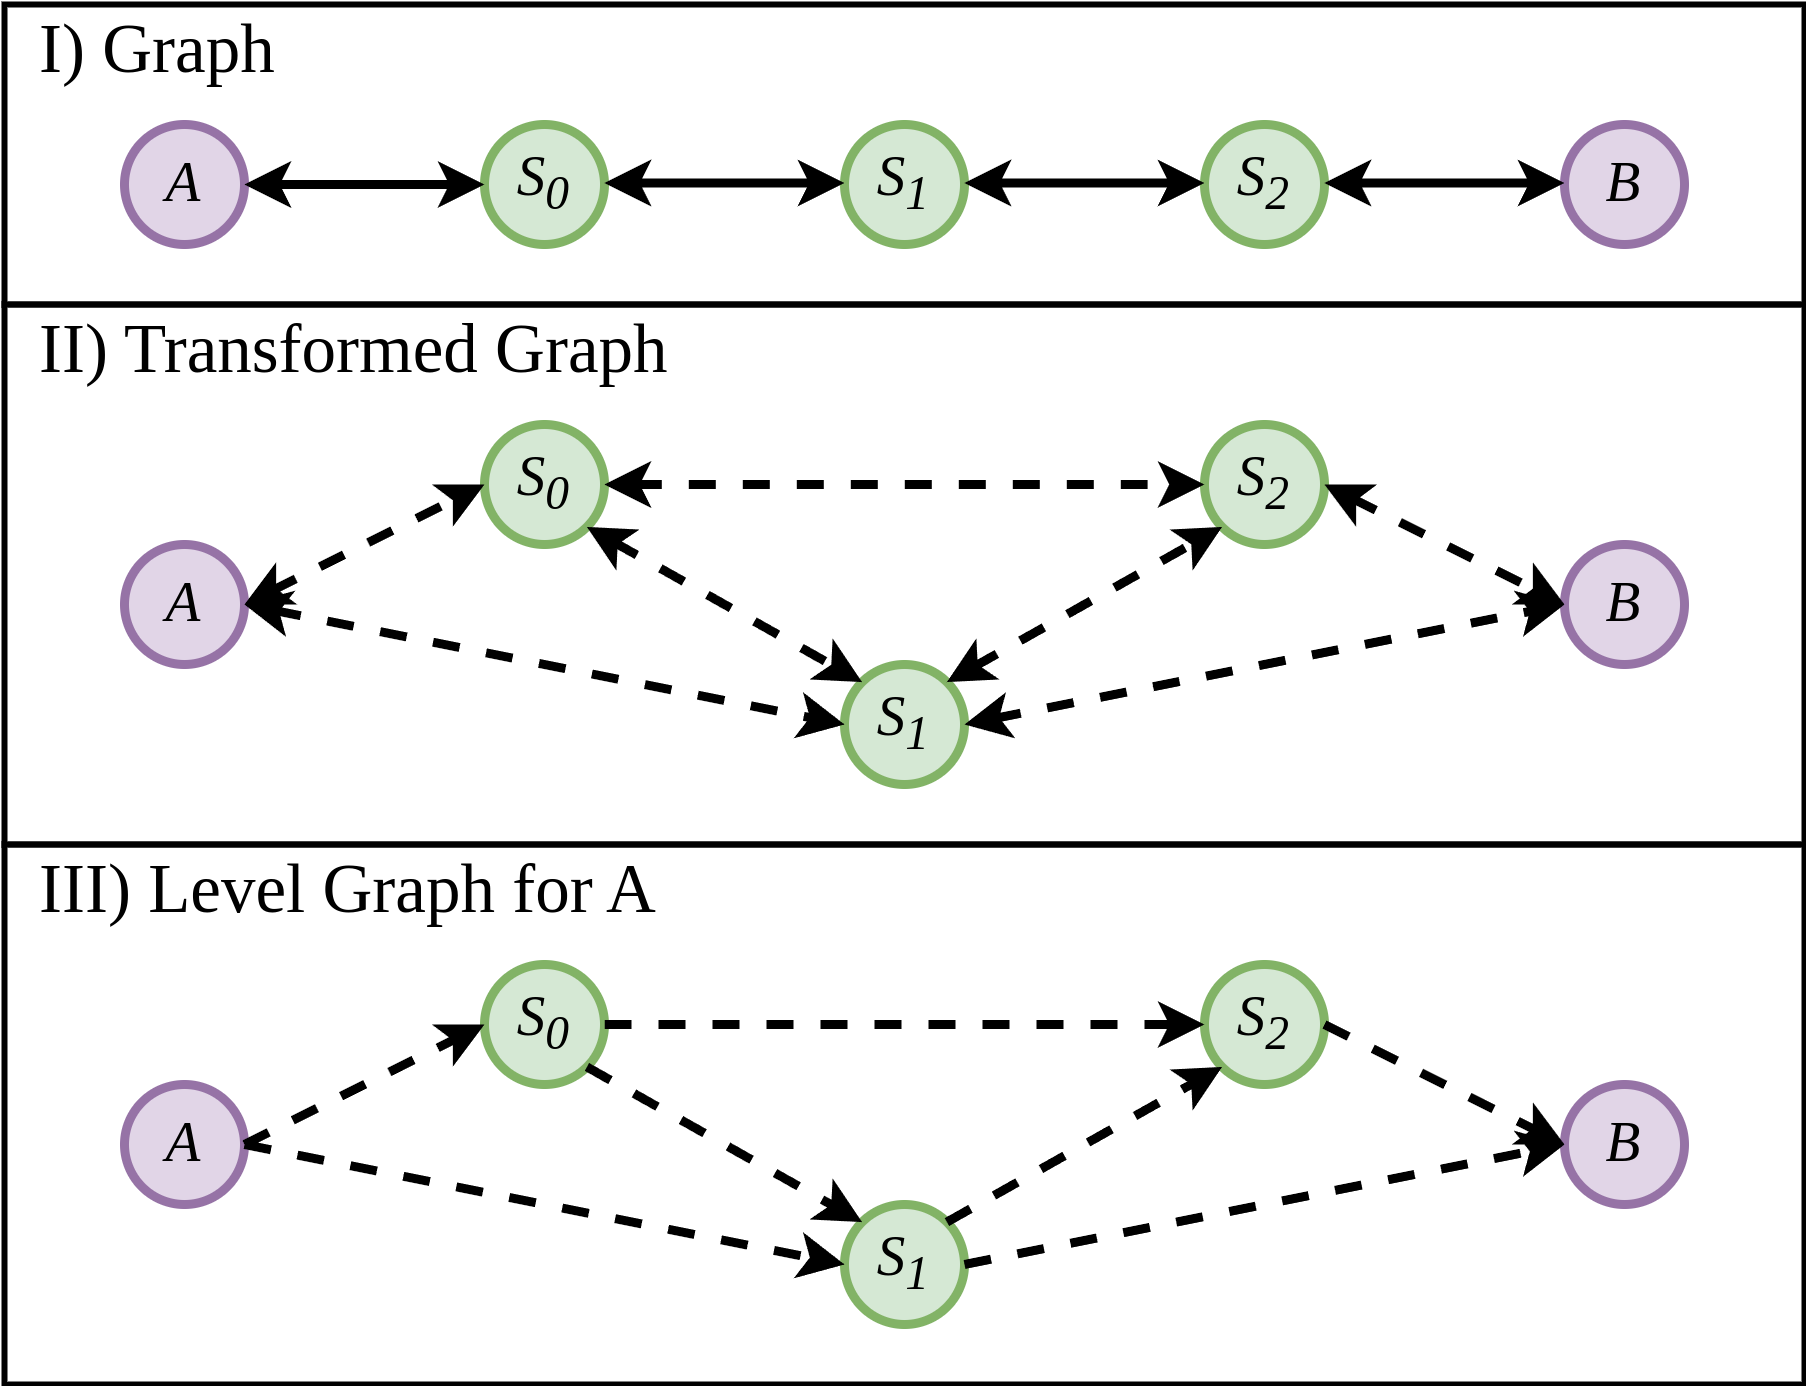
\includegraphics[width = \figurewidth]{./figures/formulation/road_charging_paths.png}
	\caption{Graphs for simple vehicular transportation network. Panel I shows a graph $G$ for a section of road from $A$ to $B$ with stations $S_0$, $S_1$, and $S_2$. Panel II shows the transformed graph $\hat{G}$ for a vehicle with sufficient range to reach $S_1$ from $A$ and $B$. Panel III shows the level graph $\overline{G}_A$ for the same vehicle leaving $A$. The simple supply-paths for pair $\langle A, B \rangle$ are $A-S_0-S_1-B$, $A-S_0-S_2-B$, $A-S_1-B$, and $A-S_1-S_2-B$.}
	\label{fig:paths}
\end{figure}

The time cost of edge $(i, j) \in \hat{E}$ is the total trip time. This includes the time required to traverse the edge and the time spent charging at a station before traversing the edge. For a vehicle with a usable \gls{ess} capacity of $\beta$ at node $i$ which contains a charger whose maximum rate is $\alpha$ the time cost for edge $(i, j)$ is

\begin{equation}
	Y^T_{(i, j)} = \tau_{(i, j)} + \begin{cases}
		f_c(\epsilon_{(i, j)}, \beta, \alpha) & \epsilon_{(i, j)} \leq \beta \\
		\infty & \epsilon_{(i, j)} > \beta
	\end{cases}
\end{equation}

where $\tau$ is edge traversal time, $\epsilon$ is edge energy consumption, and $f_c$ is a function relating energy to charging time. Charging is modeled using a CC-CV relationship. The first part of charging is linear and the second part follows an exponential decay function. The time required for a given charge event is

\begin{gather}
	\begin{gathered}
	f_{c}(\epsilon, \beta, \alpha) = \\\begin{cases}
		\frac{\epsilon}{\alpha} & \epsilon \leq \eta\beta \\
		\frac{\eta\beta}{\alpha}\left(1-\ln{\left(1-\frac{\epsilon - \eta\beta}{\beta(1-\eta)}\right)}\right) &  \epsilon > \eta\beta
	\end{cases}
	\end{gathered}
\end{gather}

where $\eta$ is the inflection point separating linear and nonlinear charging. A typical value for $\eta$ will be in the range of 0.7 to 0.8. Charging past $\eta$ will be substantially slower than below $\eta$.

The time-cost of queuing depends on the presence or absence of other vehicles at a station and is modeled at a system level. Queue waiting time is modeled using the M/M/c queuing formula. The expected queue length for an M/M/c queue is computed as

\begin{gather}
	L_q = f_{q}(\lambda, \mu, c) = \pi_0\frac{\rho(c\rho)^c}{c!(1-\rho)^2}\label{eq:w_q}\\
	\pi_0=\left[\left(\sum_{k = 0}^{c - 1}\frac{(c\rho)^k}{k!}\right) + \frac{(c\rho)^c}{c!(1 - \rho)}\right]^{-1}\\
	\rho = \frac{\lambda}{c\mu}
\end{gather}

where $\lambda$ is the mean arrival frequency, $\mu$ is the mean service frequency, $c$ is the number of homogeneous servers, $\rho$ is the ratio of arrival frequency to composite maximum service completion frequency, and $\pi_0$ is the probability of an empty system. The M/M/c formulation assumes exponential distributions for $\lambda$ and $\mu$. One can think of $\rho$ as equivalent to "utilization". Where $\rho$ is low the station has excess capacity and where high the station approaches saturation. $L_q$ approaches infinity as $\rho$ approaches one. The expected waiting in an M/M/c queue can be computed using Little's rule. Little's rule states $W_q = L_q\lambda^{-1}$ and serves as a conservation condition for a stable queue. In order for a queue to retain a stable length over a period of time, the same number of vehicles have to enter the queue as leave the queue. This means that the expected time interval between advances in the queue is $\lambda^{-1}$ and a vehicle is expected to have to endure $L_q$ advances before leaving the queue. Since the same applies to all vehicles in the queue, the total queue waiting time $\hat{W}_q$ can be computed as

\begin{gather}
	\hat{W}_q = \frac{L_q^2}{\lambda}
\end{gather}

which represents the system-level delay caused by the queue. Queue formation is a combinatorial effect. In order to maintain a stable queue length, the rate of vehicle arrivals must match the rate of vehicle departures. This is extremely unlikely over a short time interval and the length of the queue should fluctuate. Over a long enough period, a stable non-zero mean queue length can emerge even when the rate of arrivals is less than the theoretical maximum capacity of the station. This happens because the random sequence of arrivals and departures will, often, produce scenarios where all ports are occupied when the next vehicle arrives. There will be some times when there are no vehicles at the station at all and some times when a long queue exists. \textbf{Scenarios where all ports are occupied are more likely at stations with fewer ports even at identical utilization rates}. This effect is shown in Figure \ref{fig:queue}.

\begin{figure}[H]
	\centering
	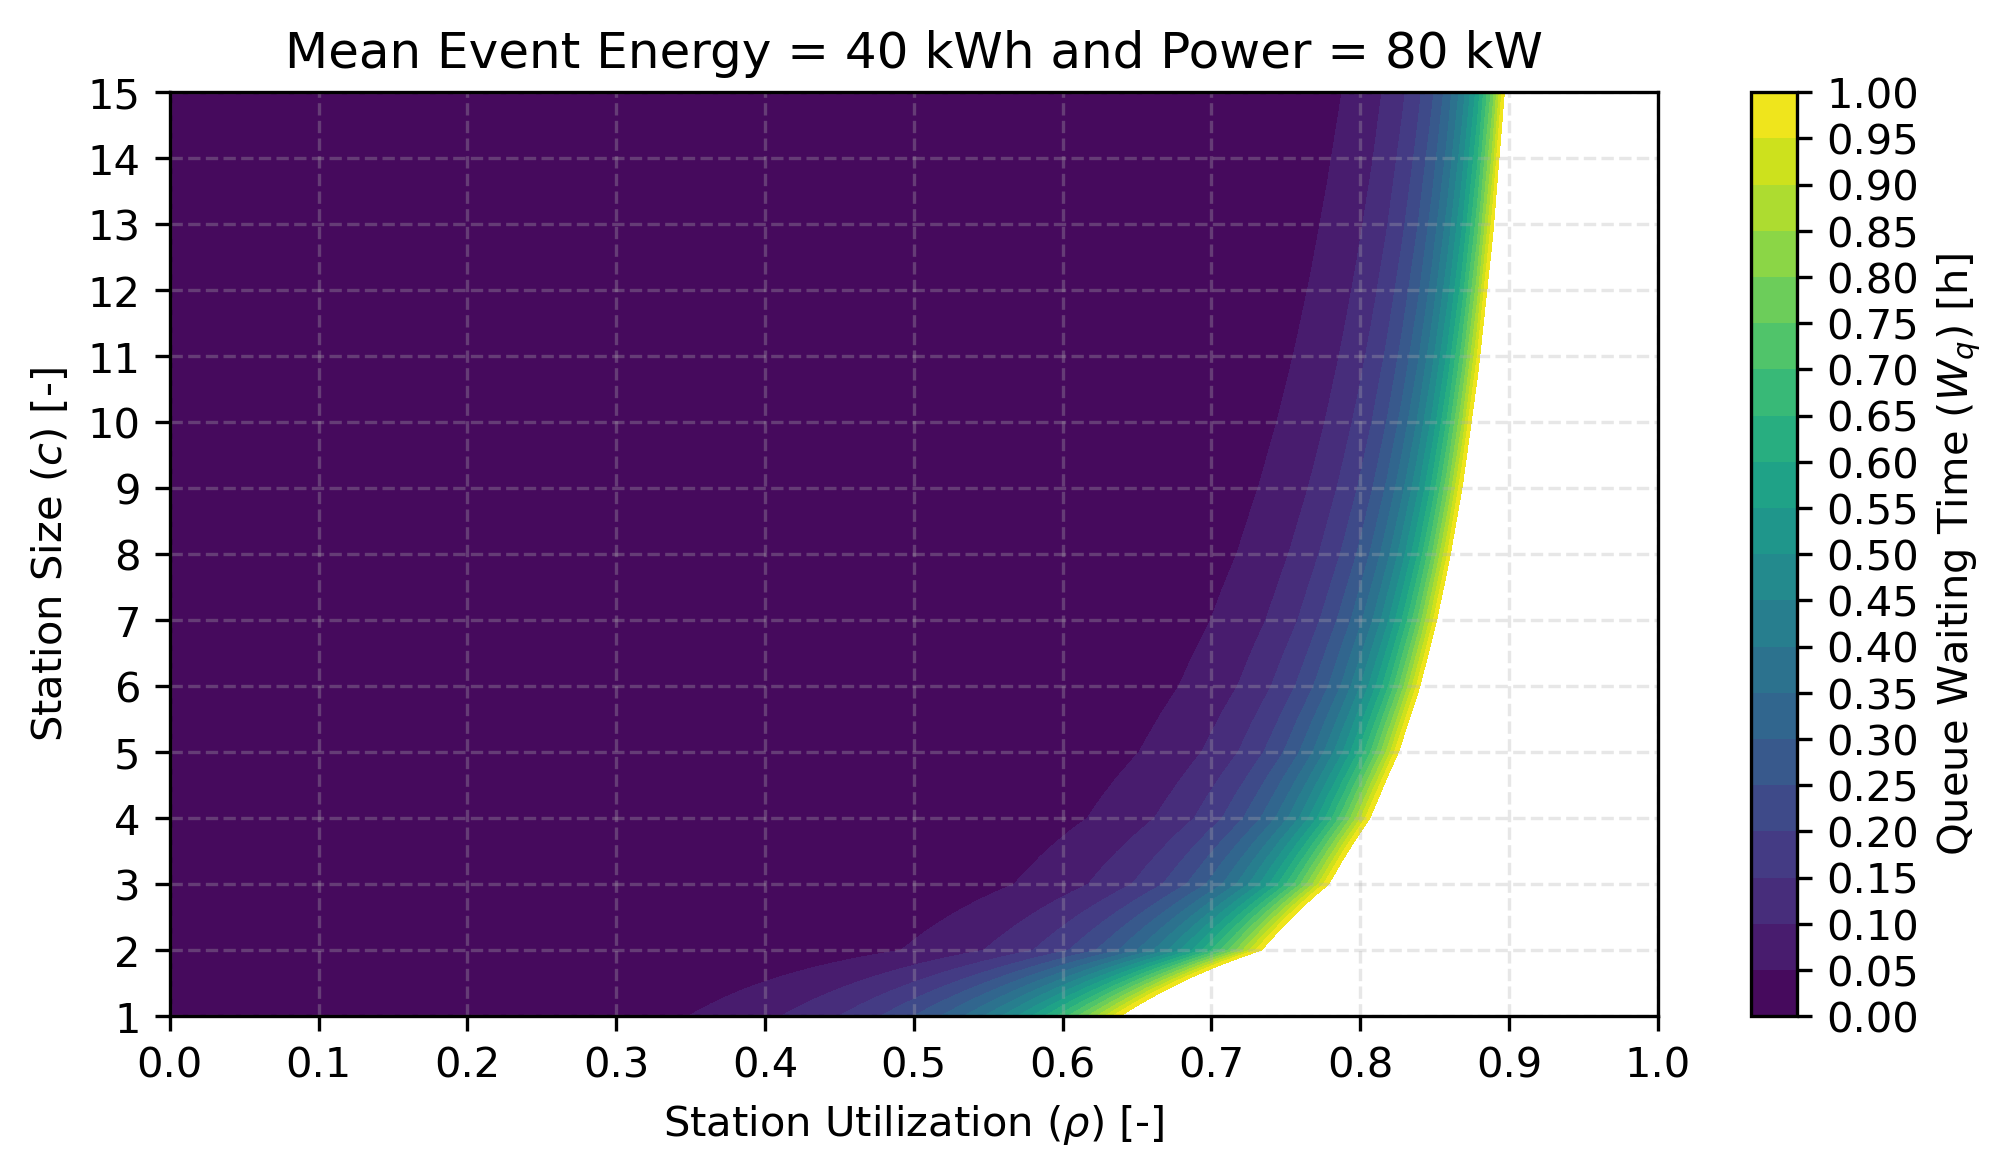
\includegraphics[width = \figurewidth]{./figures/formulation/queue.png}
	\caption{Queuing time with M/M/c queue model}
	\label{fig:queue}
\end{figure}

Queuing dynamics mean that larger stations can handle higher utilization rates. As in Figure \ref{fig:queue}, a station with 15 ports can handle a rate of $\rho = 0.8$ before substantial queue formation equivalent to 24 vehicles per hour. A station of 4 chargers can handle a rate of $\rho = 0.6$ before substantial queue formation equivalent to 4.8 vehicles per hour. Thus, larger stations are more efficient on a capacity-per-charger basis with this effect being very substantial below 10 ports and leveling off after 15 ports given current values for mean energy dispensed and charging rate.

\subsection{Formulation}

The purpose of this formulation is to minimize total travel time in the system subject to travel demand. Travel time minimization is accomplished by vehicle routing and charging station provision. For a given origin-destination pair there will, usually, be multiple viable charging paths of different lengths. As demand increases, chargers become increasingly congested leading to queuing time at stations. Queuing delays on shorter paths will push traffic to longer paths. Eventually, queuing will be sufficient to make the charging network no longer beneficial. This point is defined as when the marginal vehicle trip would take as much time using the DC network as it would take using AC charging. The goal is to place DC chargers and route \glspl{bev} to minimize system-wide total travel time. As such, each origin-destination pair has a "failure" flow which vehicles can be assigned to and the penalty assigned for this is equal to the travel time with level 1 charging.

Delay at stations is modeled using the outputs of the M/M/c queue formula as previously discussed. Specifically, the outputs are linearized by converting the nonlinear relationship between station utilization $\lambda$ and delay time $W_q$ as follows:

\begin{itemize}
	\item If the station size $c$ and expected service rate $\mu$ are held constant, then the arrival rate $\lambda$ maps directly to the utilization rate $\rho$. Define a set $K = \{k_0, k_1, \dots k_n\}$ of marginal units of $\rho$ where $\sum_{i = 0}^{N} k_i = 1$.
	\item Define $Y^V = \{y^v_0, y^v_1, \dots y^v_n\}$ as marginal units of station volume $\lambda$ corresponding to $K$.
	\item Define $Y^D = \{y^d_0, y^d_1, \dots y^d_n\}$ as marginal units of station delay $\hat{W}_q$ corresponding to $K$.
	\item Define $X^U$ as a set of unit interval constrained linear utilization variables corresponding to $K$. The marginal volume terms multiplied by the utilization variables must sum to $\lambda$ seen at the station ($\sum_{i}^{N} y^v_i x^u_i = \lambda$).
	\item The system-wide delay imposed by congestion at a station can be computed as $\sum_{i}^{N} y^d_i x^u_i$.
\end{itemize}

The linearized delay function does not require that marginal units of volume be of constant size. Rather, due to the highly nonlinear nature of the relationship, many more capacity interval size should decrease as $\rho$ approaches 1 and the delay approaches infinity. The linearized relationship between $\lambda$ and $\hat{W}_q$ at a station with 4 chargers and a half-hour expected charging time is shown in Figure \ref{fig:linearized}.

\begin{figure}[H]
	\centering
	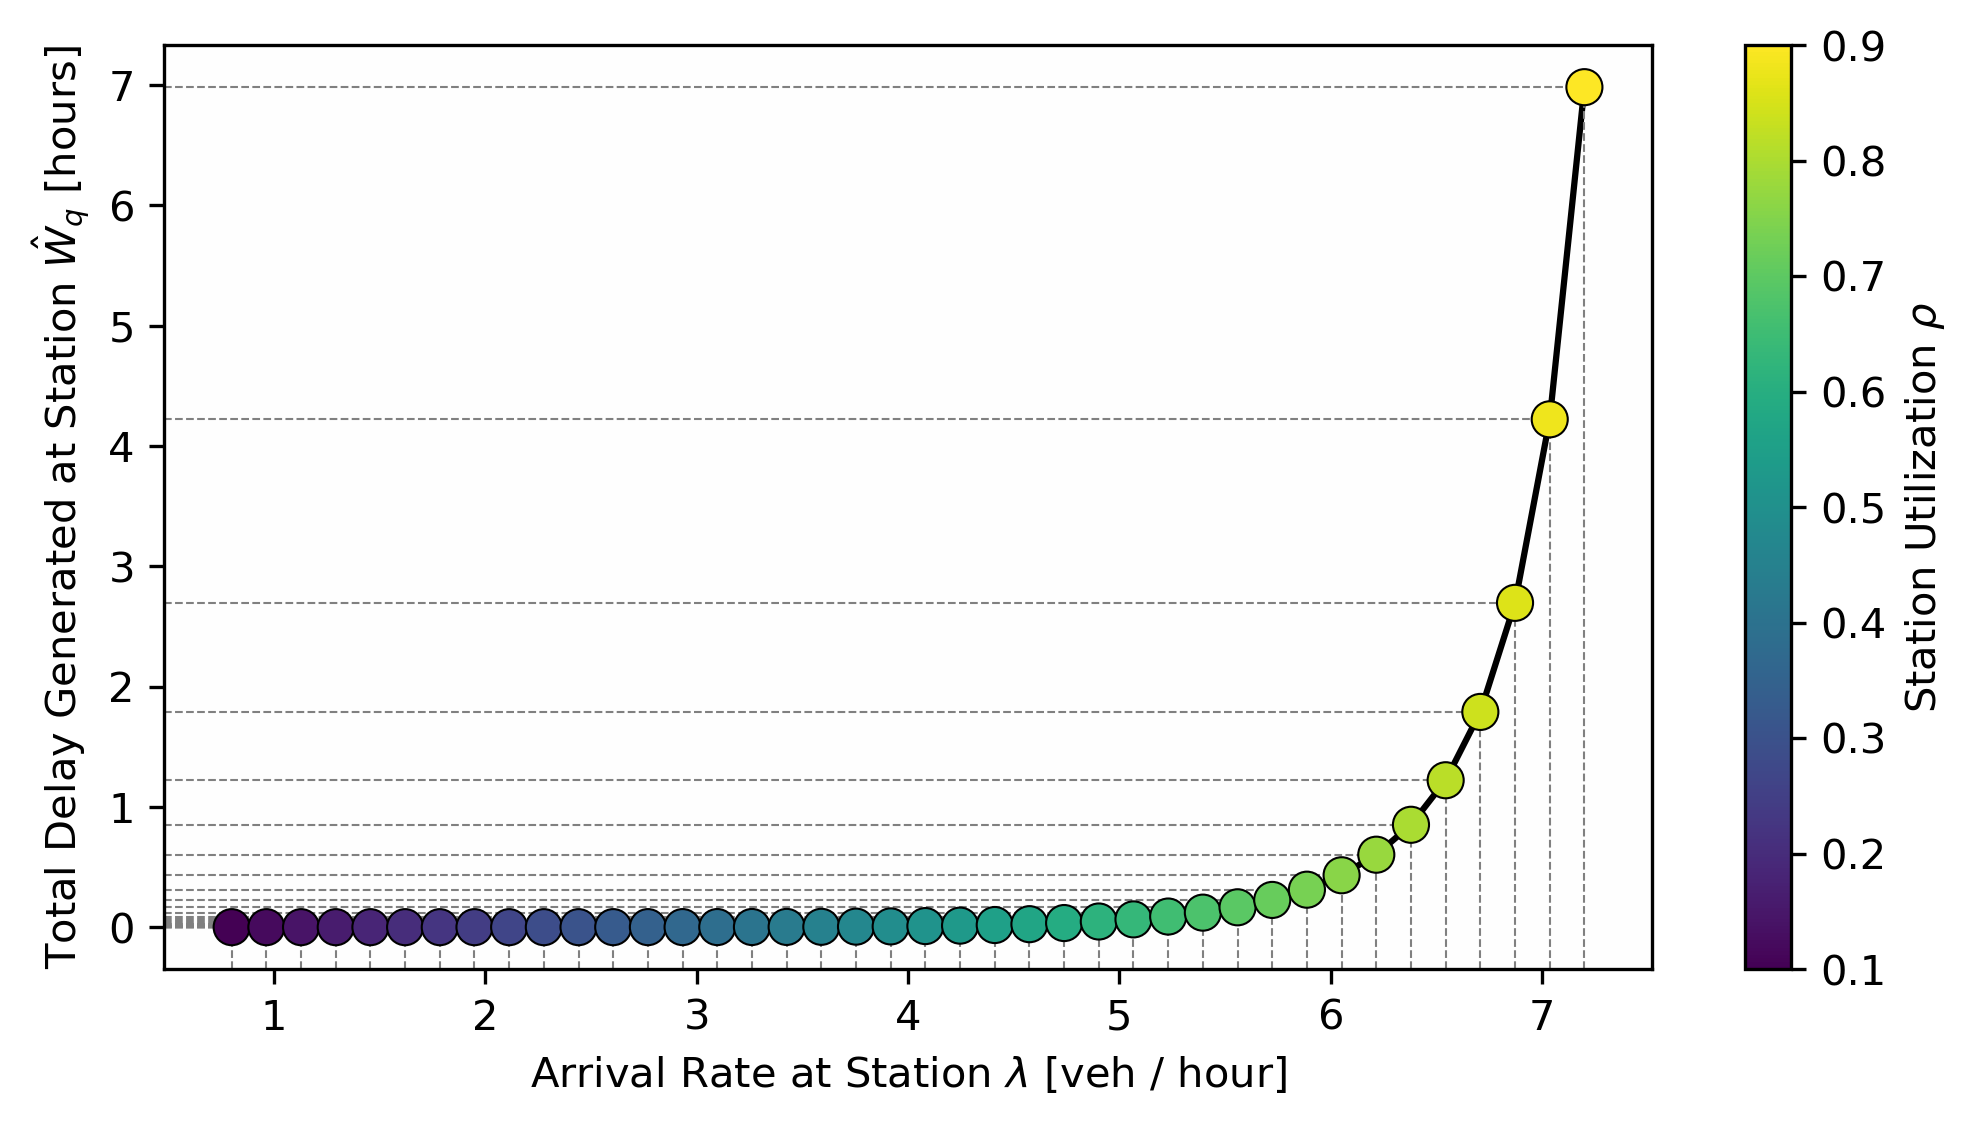
\includegraphics[width = \figurewidth]{./figures/linearized.png}
	\caption{Example linearized relationship between $\lambda$ and $\hat{W}_q$}
	\label{fig:linearized}
\end{figure}

The marginal queuing delay penalty for each utilization interval in $\Delta$ is higher than the previous interval. As a result, the optimal solution will always exhaust lower intervals before higher intervals without needing an explicit constraint. In this formulation, network flow is modeled as a continuous flow in units of vehicles per unit time. This is the same approximation as in the M/M/c queue model. Congestion depends on station size. Stations are initialized with a vector of $m$ binary variables representing possible sizes (e.g. 1 charger, 3 chargers, 5 chargers). The vector of station size binary variables must sum to 1.

Optimization uses the following sets:

\begin{itemize}
	\item $G = \{V, E\}$: System graph containing nodes $v \in V$ and edges $(i, j) \in E$. Edge costs are defined by the following sets: \begin{itemize}
		\item $Y^T$: The time required to traverse edge $(i, j)$
		%		\item $Y^E$: The time required to charge at node $i$ to successfully traverse edge $(i, j)$
	\end{itemize}
	\item $O \subseteq V$: Set of origin nodes
	\item $D \subseteq V$: Set of destination nodes
	\item $S \subseteq V$: Set of nodes with charging stations (or the possibility of a station). Stations provide energy to vehicle flows at a given rate. Depending on the utilization level of the station, vehicles may experience delay. The relationship between utilization and delay is linearized using the following sets: \begin{itemize}
		\item $C_s$: Set of possible station sizes at station $s \in S$
		\item $K_{s, c}$: Set of capacity intervals at station $s \in S$ for station size $c \in C_s$
		\item $Y^V$: Set of volumes corresponding to each $c \in C_s$ and $k \in K_s$
		\item $Y^D$: Set of delays corresponding to each $c \in C_s$ and $k \in K_s$ 
		\item $Y^C$: Set of expenditure requirements to install a given number of chargers at a given station.
	\end{itemize}
	\item $\hat{C}$: Maximum number of chargers which can be installed
	\item $Q$: Set of demand tuples of the form $\langle o, d, v, c, \hat{t} \rangle$ where $o$ is the origin, $d$ is the destination, $v$ is the volume, $c$ is the capacity of the \gls{ess} capacity of vehicles, and $\hat{t}$ is the maximum travel time that is acceptable for the given demand. \begin{itemize}
		\item $Y^Q$: Set of time penalties for failing to accommodate flow. Set so that $y^q_q$ is equal to $\hat{t}$ in $q$.
	\end{itemize}
	\item $P$: Set of paths corresponding to each demand $q \in Q$. Paths begin at $o \in O$ and end at $d \in D$. All intermediate nodes $i \in P \setminus \{o, d\}$ must be stations $s \in S$.\begin{itemize}
		\item $P^q$: Paths that correspond to demand $q \in Q$
		\item $P^s$: Paths that include station $s \in S$
	\end{itemize}
	\item $X$: Set of continuous decision variables: \begin{itemize}
		\item $X^Q$: Portion of demand flow not facilitated by the network
		\item $X^P$: Flow volumes along paths
		\item $X^U$: Portion of station capacity intervals utilized
		\item $X^V$: Volume seen at station
		\item $X^D$: Queuing delay seen at station
	\end{itemize}
	\item $U$: Set of integer decision variables: \begin{itemize}
		\item $U^S$: Booleans for station sizes corresponding to $S$ and $C$
	\end{itemize}
\end{itemize}


The objective of the optimization is

\begin{gather}
	\begin{gathered}
	\min_{\overline{X},\overline{U}}\quad \underbrace{\sum_{q \in Q} x^q_qy^q_q}_{\text{Penalty Time}} + \underbrace{\sum_{q \in Q}\sum_{P^q \in P}\sum_{p \in P^q}\sum_{(i, j) \in p} x^p_py^t_{(i, j)}}_{\text{Edge Traversal Time}} \\+ \underbrace{\sum_{s \in S}\sum_{c \in C_s}
		\sum_{k \in K_{s, c}} u^s_{s, c}x^u_{s, c, k}y^d_{s, c, k}}_{\text{Queuing Time}} \label{eq:tm:obj}
	\end{gathered}
\end{gather}

subject to

\begin{gather}
	q[v] - x^q_q - \sum_{p \in P^q}x^p_p = 0 \quad \forall q \in Q \label{eq:tm:flow_dem} \\
	\sum_{p \in P^s} x^p_p - \sum_{c \in C_s}
	\sum_{k \in K_{s, c}} u^s_{s, c}x^u_{s, c, k}y^v_{s, c, k} = 0 \quad \forall s \in S \label{eq:tm:flow_cons} \\
	x^u_{s, c, k} - u^s_{s, c} \leq 0 \quad \forall s \in S, \ \forall c \in C_s,\ \forall k\in K_{s, c} \label{eq:tm:sz_int} \\
	\sum_{c \in C_s} u^s_{s, c} - 1 = 0 \quad \forall s \in S \label{eq:tm:chg_unity} \\
	\sum_{s \in S}\sum_{c \in C_s} y^c_{s, c}u^s_{s, c} - \hat{C} \leq 0 \label{eq:tm:chg_tot}
\end{gather}

The objective function \eqref{eq:tm:obj} minimizes total travel time in three terms. The first term is the time penalties accrued for failing to accommodate demand. The theory is that, without adequate DC charging infrastructure, vehicles could, theoretically, complete the trip using AC charging or a different mode but these would impose a cost penalty. The second term is the time spent charging to and driving along edges. The third term is the time spend queuing for a charger. Constraint \eqref{eq:tm:flow_dem} forces the sum of flows and penalty flows to be equal to total volume for each demand. Constraint \eqref{eq:tm:flow_cons} forces the sum of utilization variables at a station to be equal to the sum of flows which pass through the station. Constraint \eqref{eq:tm:sz_int} forces station utilization to only accrue for the selected station size. Constraint \eqref{eq:tm:chg_unity} forces only one station size to be selected per station and \eqref{eq:tm:chg_tot} limits the total number of chargers added to the network. This formulation can be used for two varieties of analysis.

\begin{description}
	\item [Performance of Current System:] If all Booleans in $U^S$ are fixed to reflect an existing system, the result of the optimization will be the best possible performance of the existing system for a given demand level.
	\item [Optimal Expansion:] If the Booleans in $U^S$ are allowed to be changed by the optimizer, the result of the optimization will be the best possible allocation of resources to facilitate travel for a given demand level.
\end{description}

Taking the example simple network from Figure \ref{fig:paths}, one can intuit that, if each additional charger at each station is of the same cost ($Y^C_{s, c} = 1\ \forall s\in S,\ c\in C_s$), the optimal solution will be to place all available resources at the central station $S_1$ because only it can be reached from both $A$ and $B$. Doing so will give the greatest benefit in terms of queuing efficiency. The costs of adding and removing chargers may scale in a nonlinear manner. It is easy to imagine a scenario where a network operator finds it easier to remove an existing charger than to install a new charger. Re-allocating equipment between stations in a network is unlikely to be a net-zero cost operation. In such a case, the network may or may not be altered.
\section{Case Study}

%\subsection{Highway Corridor Capacity}

The state of California has large population concentrations in its northern and southern regions. These regions are connected by a highway corridor which runs through more sparsely populated agricultural areas in the San Joaquin Valley in the center of the state. Most road traffic between the states densely populated regions will follow a road corridor defined by Interstate 5 to the west and CA-99 to the east. This corridor is referred to as the 5-99 Corridor. The 5-99 corridor and all California cities with a population of greater than or equal to 50 thousand are shown in Figure \ref{fig:places_corridor}.

\begin{figure}[H]
	\centering
	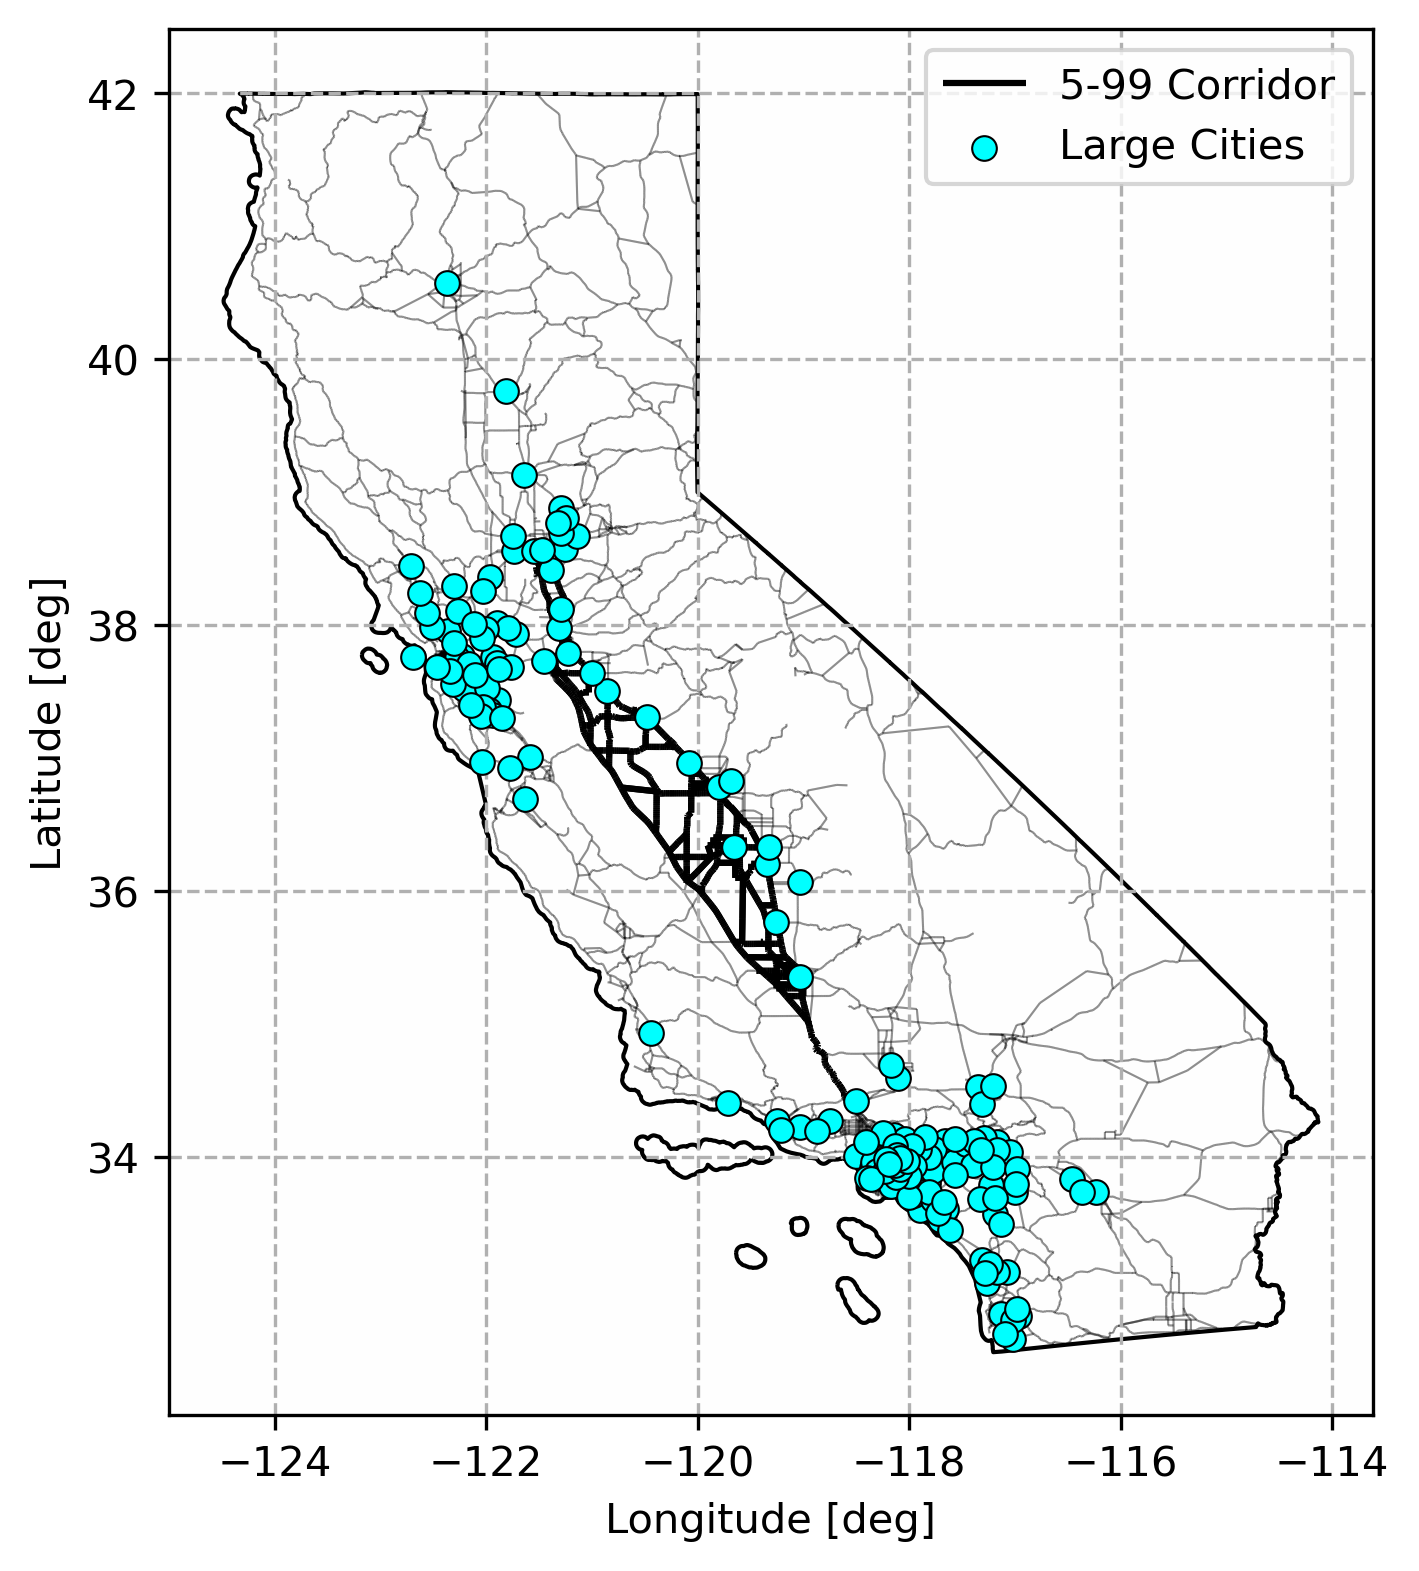
\includegraphics[width = \figurewidth]{./figures/places_corridor.png}
	\caption{5-99 Corridor and California Cities with $\geq 50,000$ population.}
	\label{fig:places_corridor}
\end{figure}

The 5-99 corridor is of vital importance to road traffic in the state of California. Because of the large distance covered by the corridor, most \glspl{bev} will have to charge at a DC charging station in order to complete their itineraries in a reasonable amount of time. DC Charging stations can be divided into those which use the CCS plug and those which use the Tesla/NACS plug. At present, there are 344 CCS and 47 NACS stations in the 5-99 corridor per AFDC \citep{afdc_2023} with 1,029 and 901 chargers respectively. Some vehicles will be limited to using only one plug type while some may use either. The locations and port counts for the CCS and NACS stations are shown in Figure \ref{fig:stations_corridor}.

\begin{figure}[H]
	\centering
	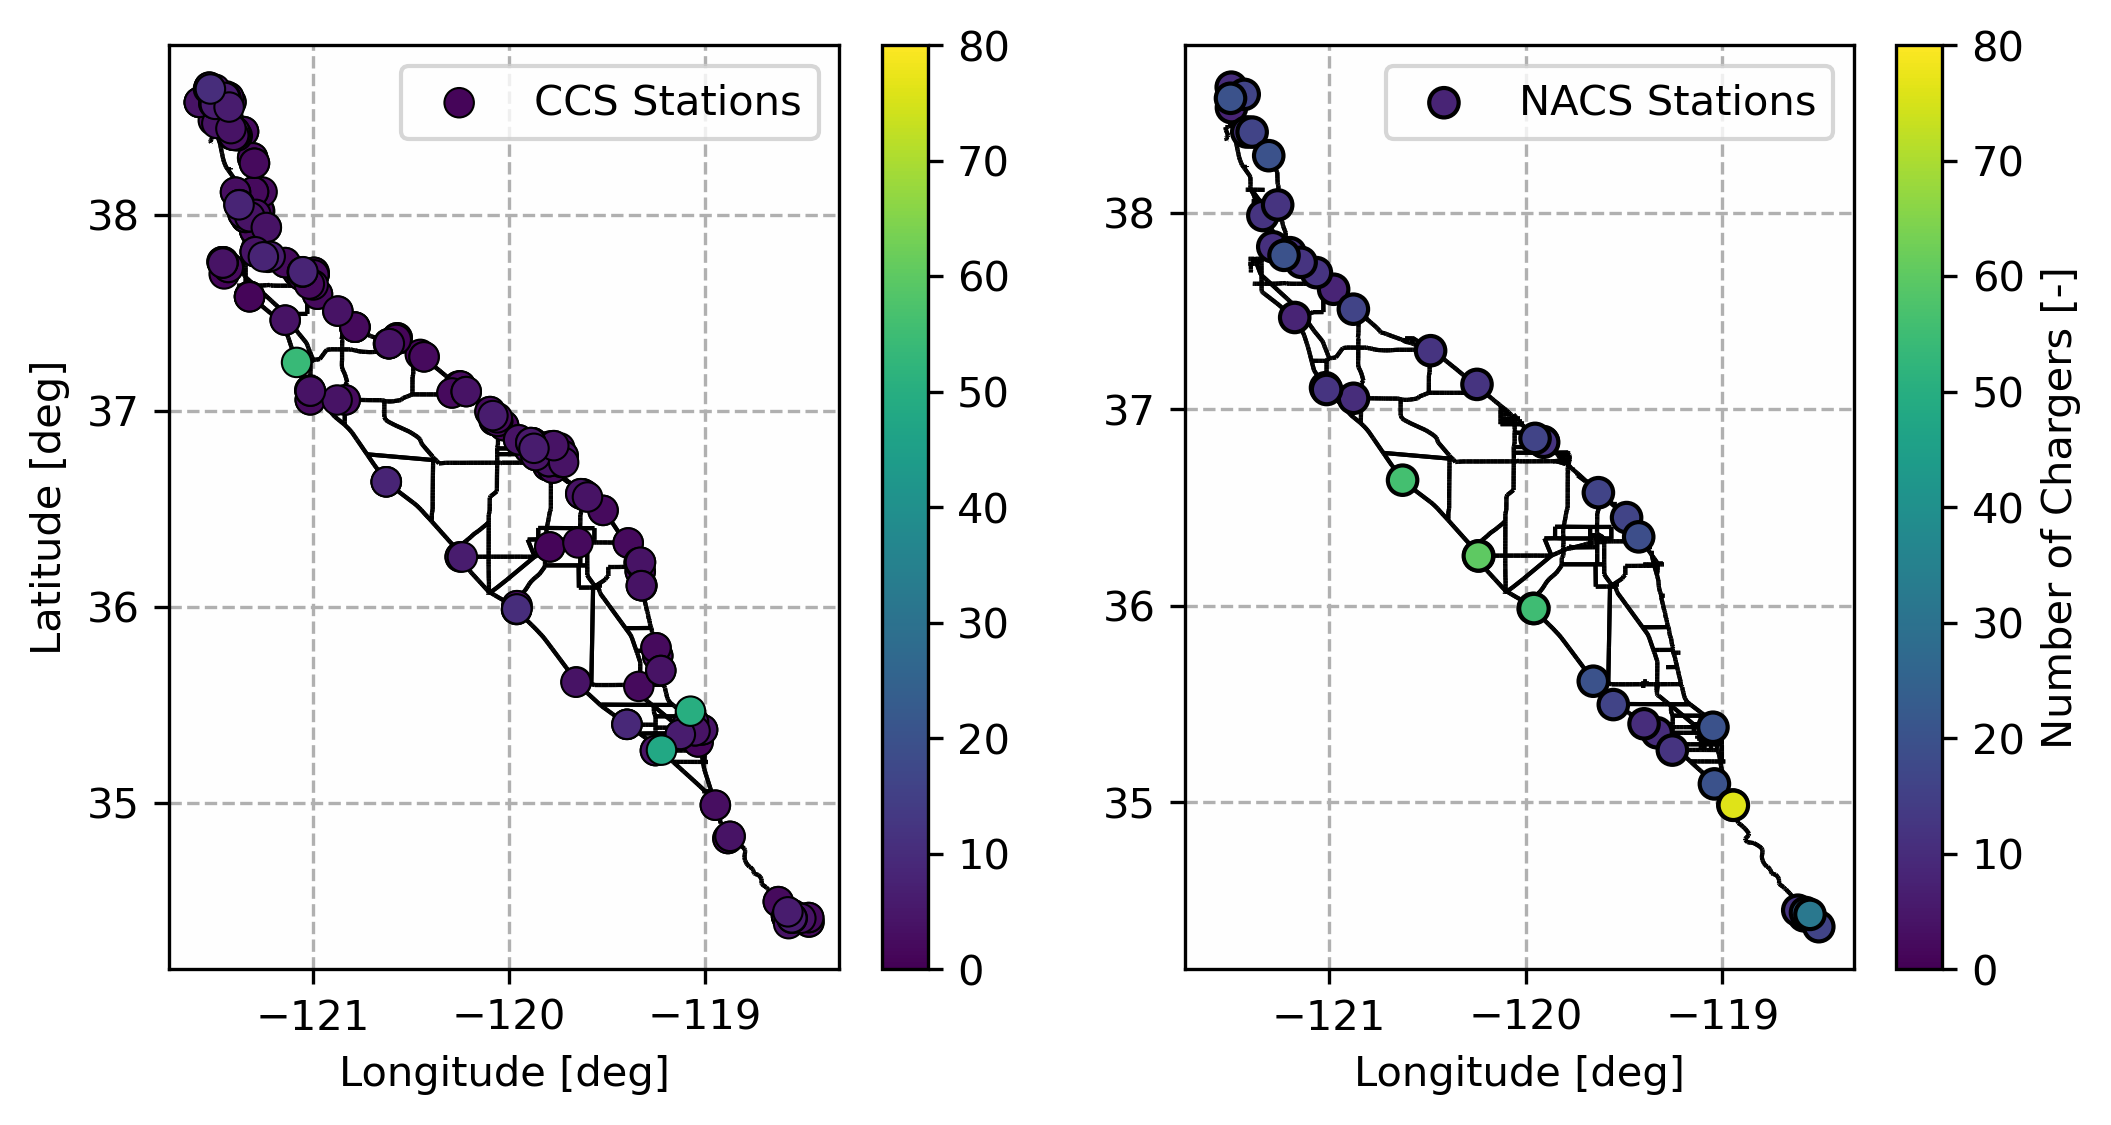
\includegraphics[width = \figurewidth]{./figures/stations_corridor.png}
	\caption{Locations and sizes of DC charging stations up to 20 chargers in 5-99 Corridor.}
	\label{fig:stations_corridor}
\end{figure}

The NACS stations in the 5-99 corridor are, in general, larger and further apart than the CCS stations. Survival functions for station size by plug type are shown in Figure \ref{fig:stations_survival}.

\begin{figure}[H]
	\centering
	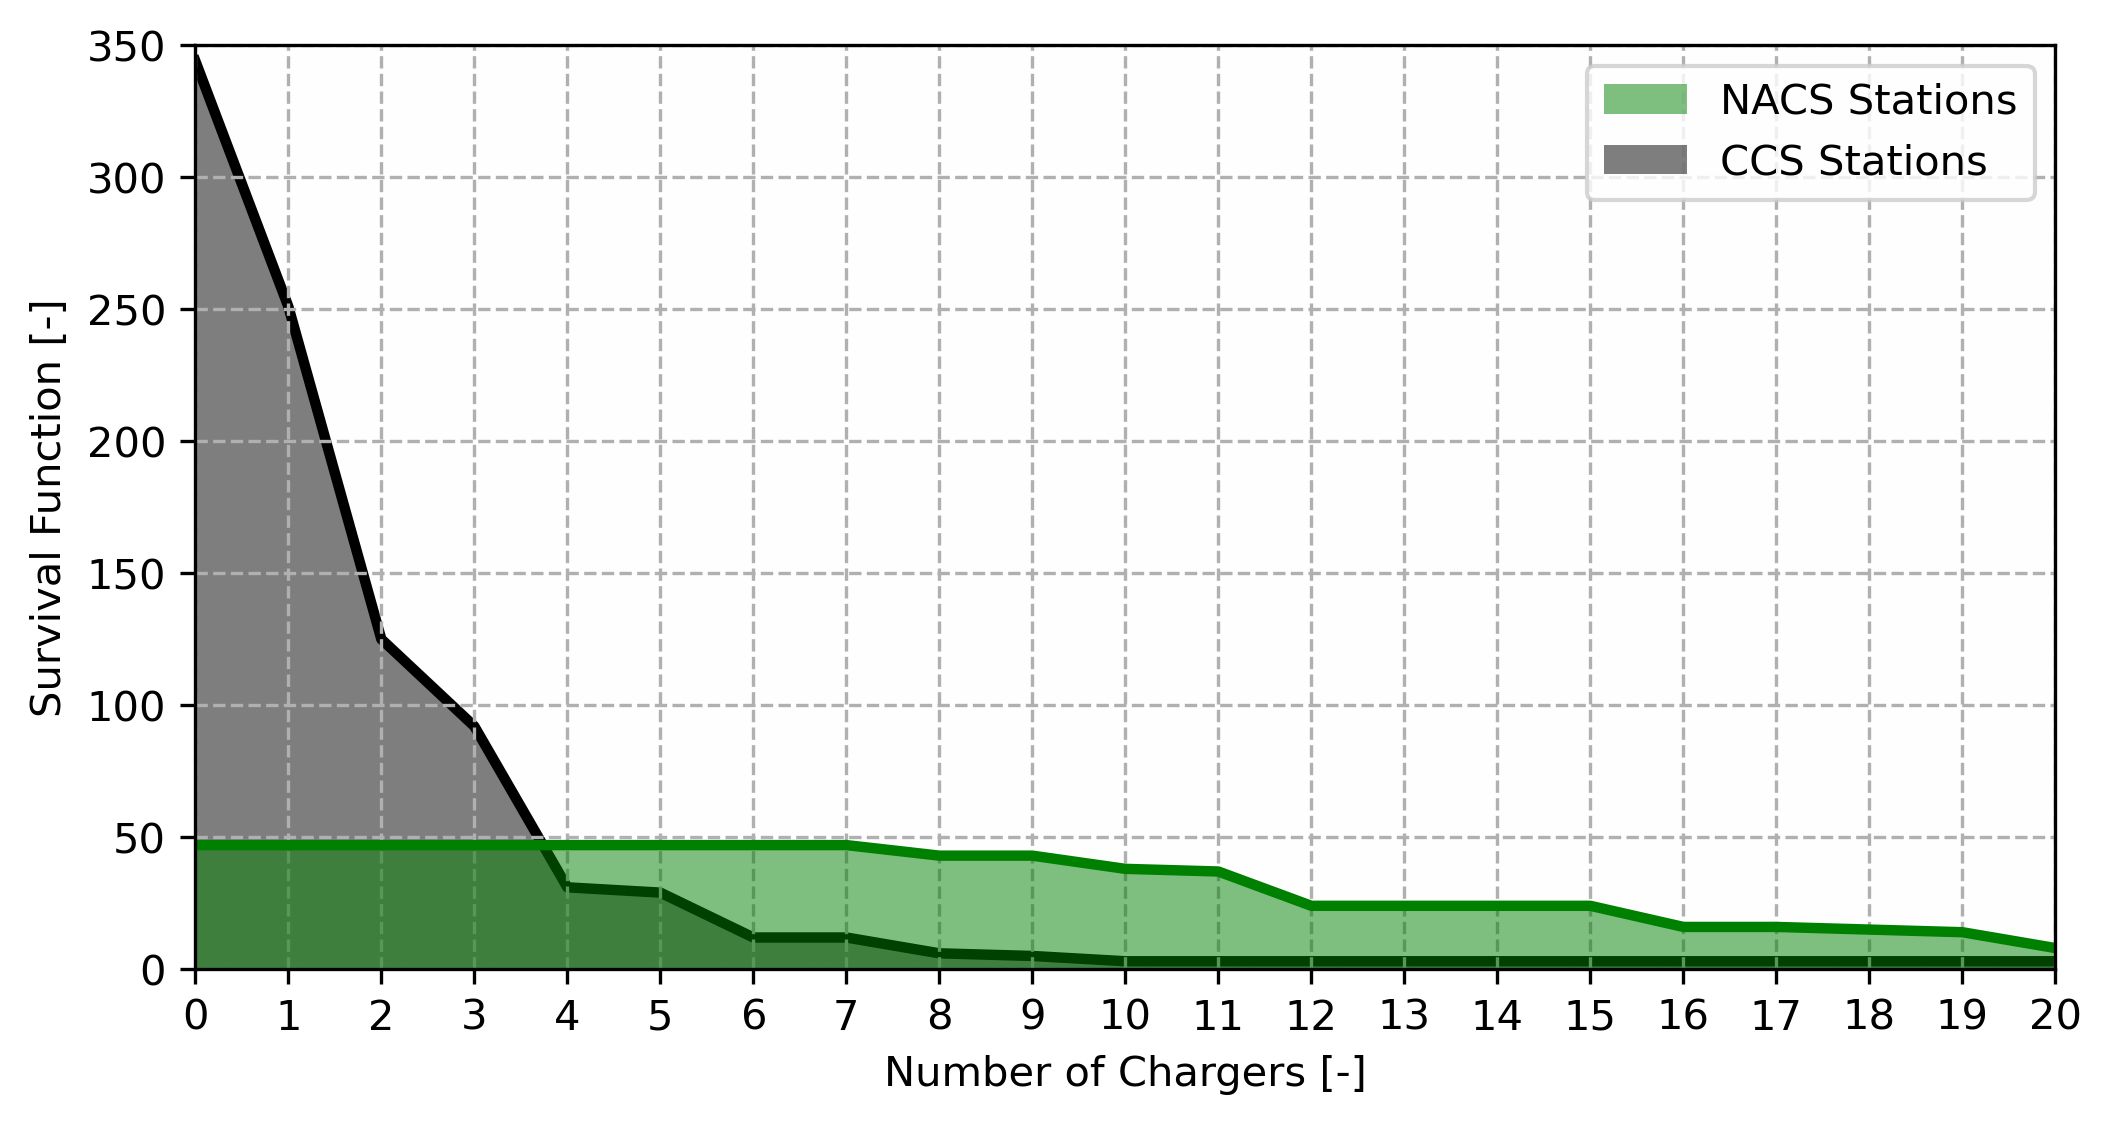
\includegraphics[width = \figurewidth]{./figures/stations_survival.png}
	\caption{Survival functions for 5-99 corridor station size (port count) by plug type.}
	\label{fig:stations_survival}
\end{figure}

A second difference is charging speeds. Tesla chargers and vehicles are capable of charging at high rates, most commonly 150 kW or 250 kW. Non-Tesla chargers frequently have maximum charging rates in the range of 50 kW to 80 kW. In the 5-99 corridor, the vast majority of the Tesla chargers are of the 250 kW variety while 60\% of CCS chargers have maximum rates less than 150 kW and 80\% less than 250 kW. Vehicles which use the CCS infrastructure may also act as a charging speed bottleneck, often with maximum charging rates lower than that of the charger \citep{AFDC_EVs_2023}. It is worth noting that charging station installation costs scale positively with peak power and negatively with number of ports \citep{Nicholas_2019}. 

A first question is how much travel can the current \gls{esn} accommodate. In order to answer this it is necessary to predict travel demand. Inter-city travel demand was generated using a travel gravity model. Populations were taken from the US Census Bureau \citep{uscb_2023_doc} and a friction function was fitted from NHTS Long Trip Survey data \citep{fhwa_2022}. The distances used for the gravity model were based on the shortest-time-paths between cities. Where a shortest path did not go through the 5-99 corridor (between San Francisco and San Jose as an example), or the shortest path was short enough to not require charging (Sacramento to Stockton for example) the demand for that pair was not considered in the optimization. The vehicle range used was 300 km, a typical practical range for a modern \gls{bev} \cite{ev_database_2025_range}. The remaining demands were converted into fractions of overall demand such that they could scale with overall demand. Following this, for those origin-destination pairs remaining, a maximum acceptable travel time was computed by computing the time the shortest path would take if the vehicle could charge at any location at a low rate (3.3 kW). If congestion causes travel times exceed this level, then the DC \gls{esn} is no longer providing benefit and the demand is considered to be un-accommodated.

Using demand fractions generated by the gravity model, the performances of the \glspl{esn} subject to varying levels of demand were computed. Metrics of performance are the mean travel-time in the system and the portion of demands accommodated. As overall demand increases, the average travel time increases due to station congestion and route detours. As a result, a larger portion of demands are not able to be accommodated and are forced to mode-switch. The optimal performances of the CCS, NACS, and combined \glspl{esn} with increasing demand is displayed in Figure \ref{fig:esn_performance}.

\begin{figure}[H]
	\centering
	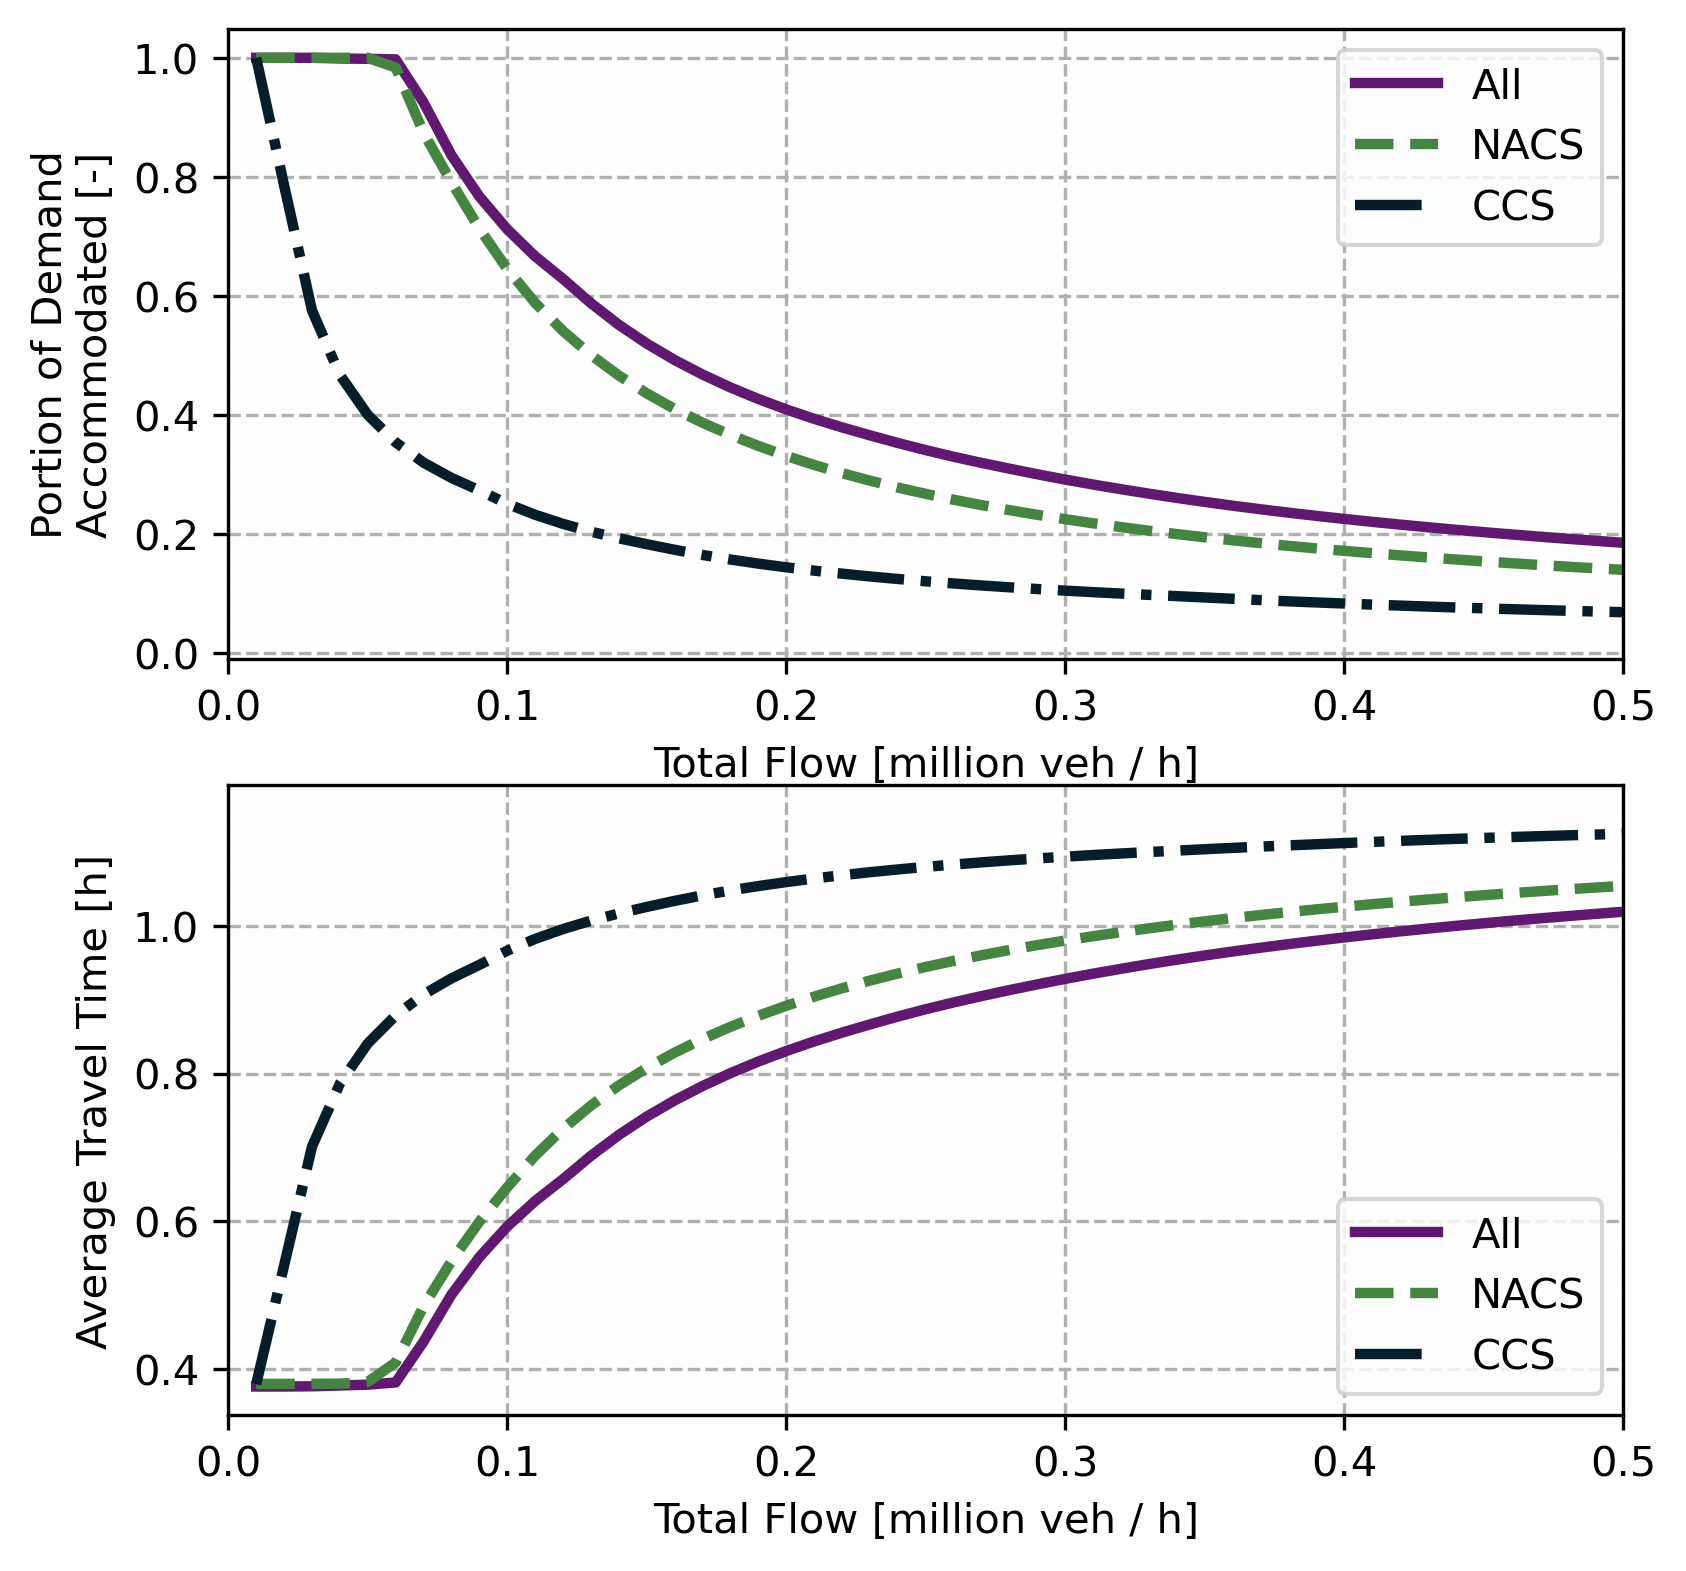
\includegraphics[width = \figurewidth]{./figures/esn_performance.png}
	\caption{Performance of CCS, NACS, and combined \glspl{esn} with increasing demand.}
	\label{fig:esn_performance}
\end{figure}

Initially, as demand increases, the extra demand can be spread to unoccupied stations without requiring queuing or re-routing. Eventually, increasing demand will require queuing, re-routing, and mode-switching. Finally, the network will not be able to accommodate any more demand and the the average travel-time will converge. The level of overall demand below which no travel-time increases are seen can be thought of as the "free-flow" capacity of the \gls{esn}. The level of overall demand which causes travel-time to converge can be thought of as the "saturation" capacity of the \gls{esn}. The range of demand used in Figure \ref{fig:esn_performance} is reflective of the range of hourly vehicle flows seen on Interstate 5 in the San Joaquin Valley \cite{caltrans_2017, caltrans_2023}. At the end of 2023, \glspl{bev} accounted for around 4\% of the California light-duty vehicle fleet \citep{cec_2024} and, likely a similar portion of light-duty vehicle trips. At this volume, some congestion should be seen at CCS stations but very little should be seen at NACS stations and this appears to be the case \citep{ucd_2024} although data is very hard to come by. The model presented, and what data can be found, suggest that the configuration of the NACS \gls{esn} is more efficient on a effective-capacity-per-charger basis. Some of the delta is based on the difference in charger speeds which favors the NACS \gls{esn}. The majority of the difference is due to the more centralized structure of the NACS network, being composed of more efficient stations. The differences in station size distribution between the CCS and NACS networks are stark. Both networks have a small number of very large stations clearly intended for high volume usage. The main difference is that the remainder of NACS stations are mid-sized, in the range of 10 to 25 chargers, while the remainder of CCS stations are small, in the range of 1 to 4 chargers.

The benefit of a more distributed network is that, by virtue of having more station locations, it is more likely to have a station closer to a demand node and to require fewer and shorter deviations out-of-path for travel demand. There are also more candidate locations which can accommodate a smaller station. The stations located in the 5-99 corridor serve local demand as well as thru-traffic, local demand may even be their primary purpose. As seen in \citep{Liu_2023}, larger stations are also favored for nodal demand if queuing is considered. However, drivers looking to charge their vehicles then return to their starting location can only go so far before the energy expended on the return leg renders the trip pointless. This means that more and better sited locations bring a real benefit. The preference for large stations is more pronounced for travel demand. Given modern \gls{bev} ranges and the concentration of long-distance traffic on limited access highways, long-distance travelers are less sensitive to the location advantages of smaller stations but benefit from the greater queue dissipation efficiency of larger stations.

A planner might be interested to know how the CCS network could be improved to perform more similarly to the NACS network given a limited budget. To answer this question, the CCS network was optimally expanded for budgets of 10, 25, 50, and 100 chargers to be assigned to existing stations. The locations and scales of additions are shown in Figure \ref{fig:augmented_esns}.

\begin{figure}[H]
	\centering
	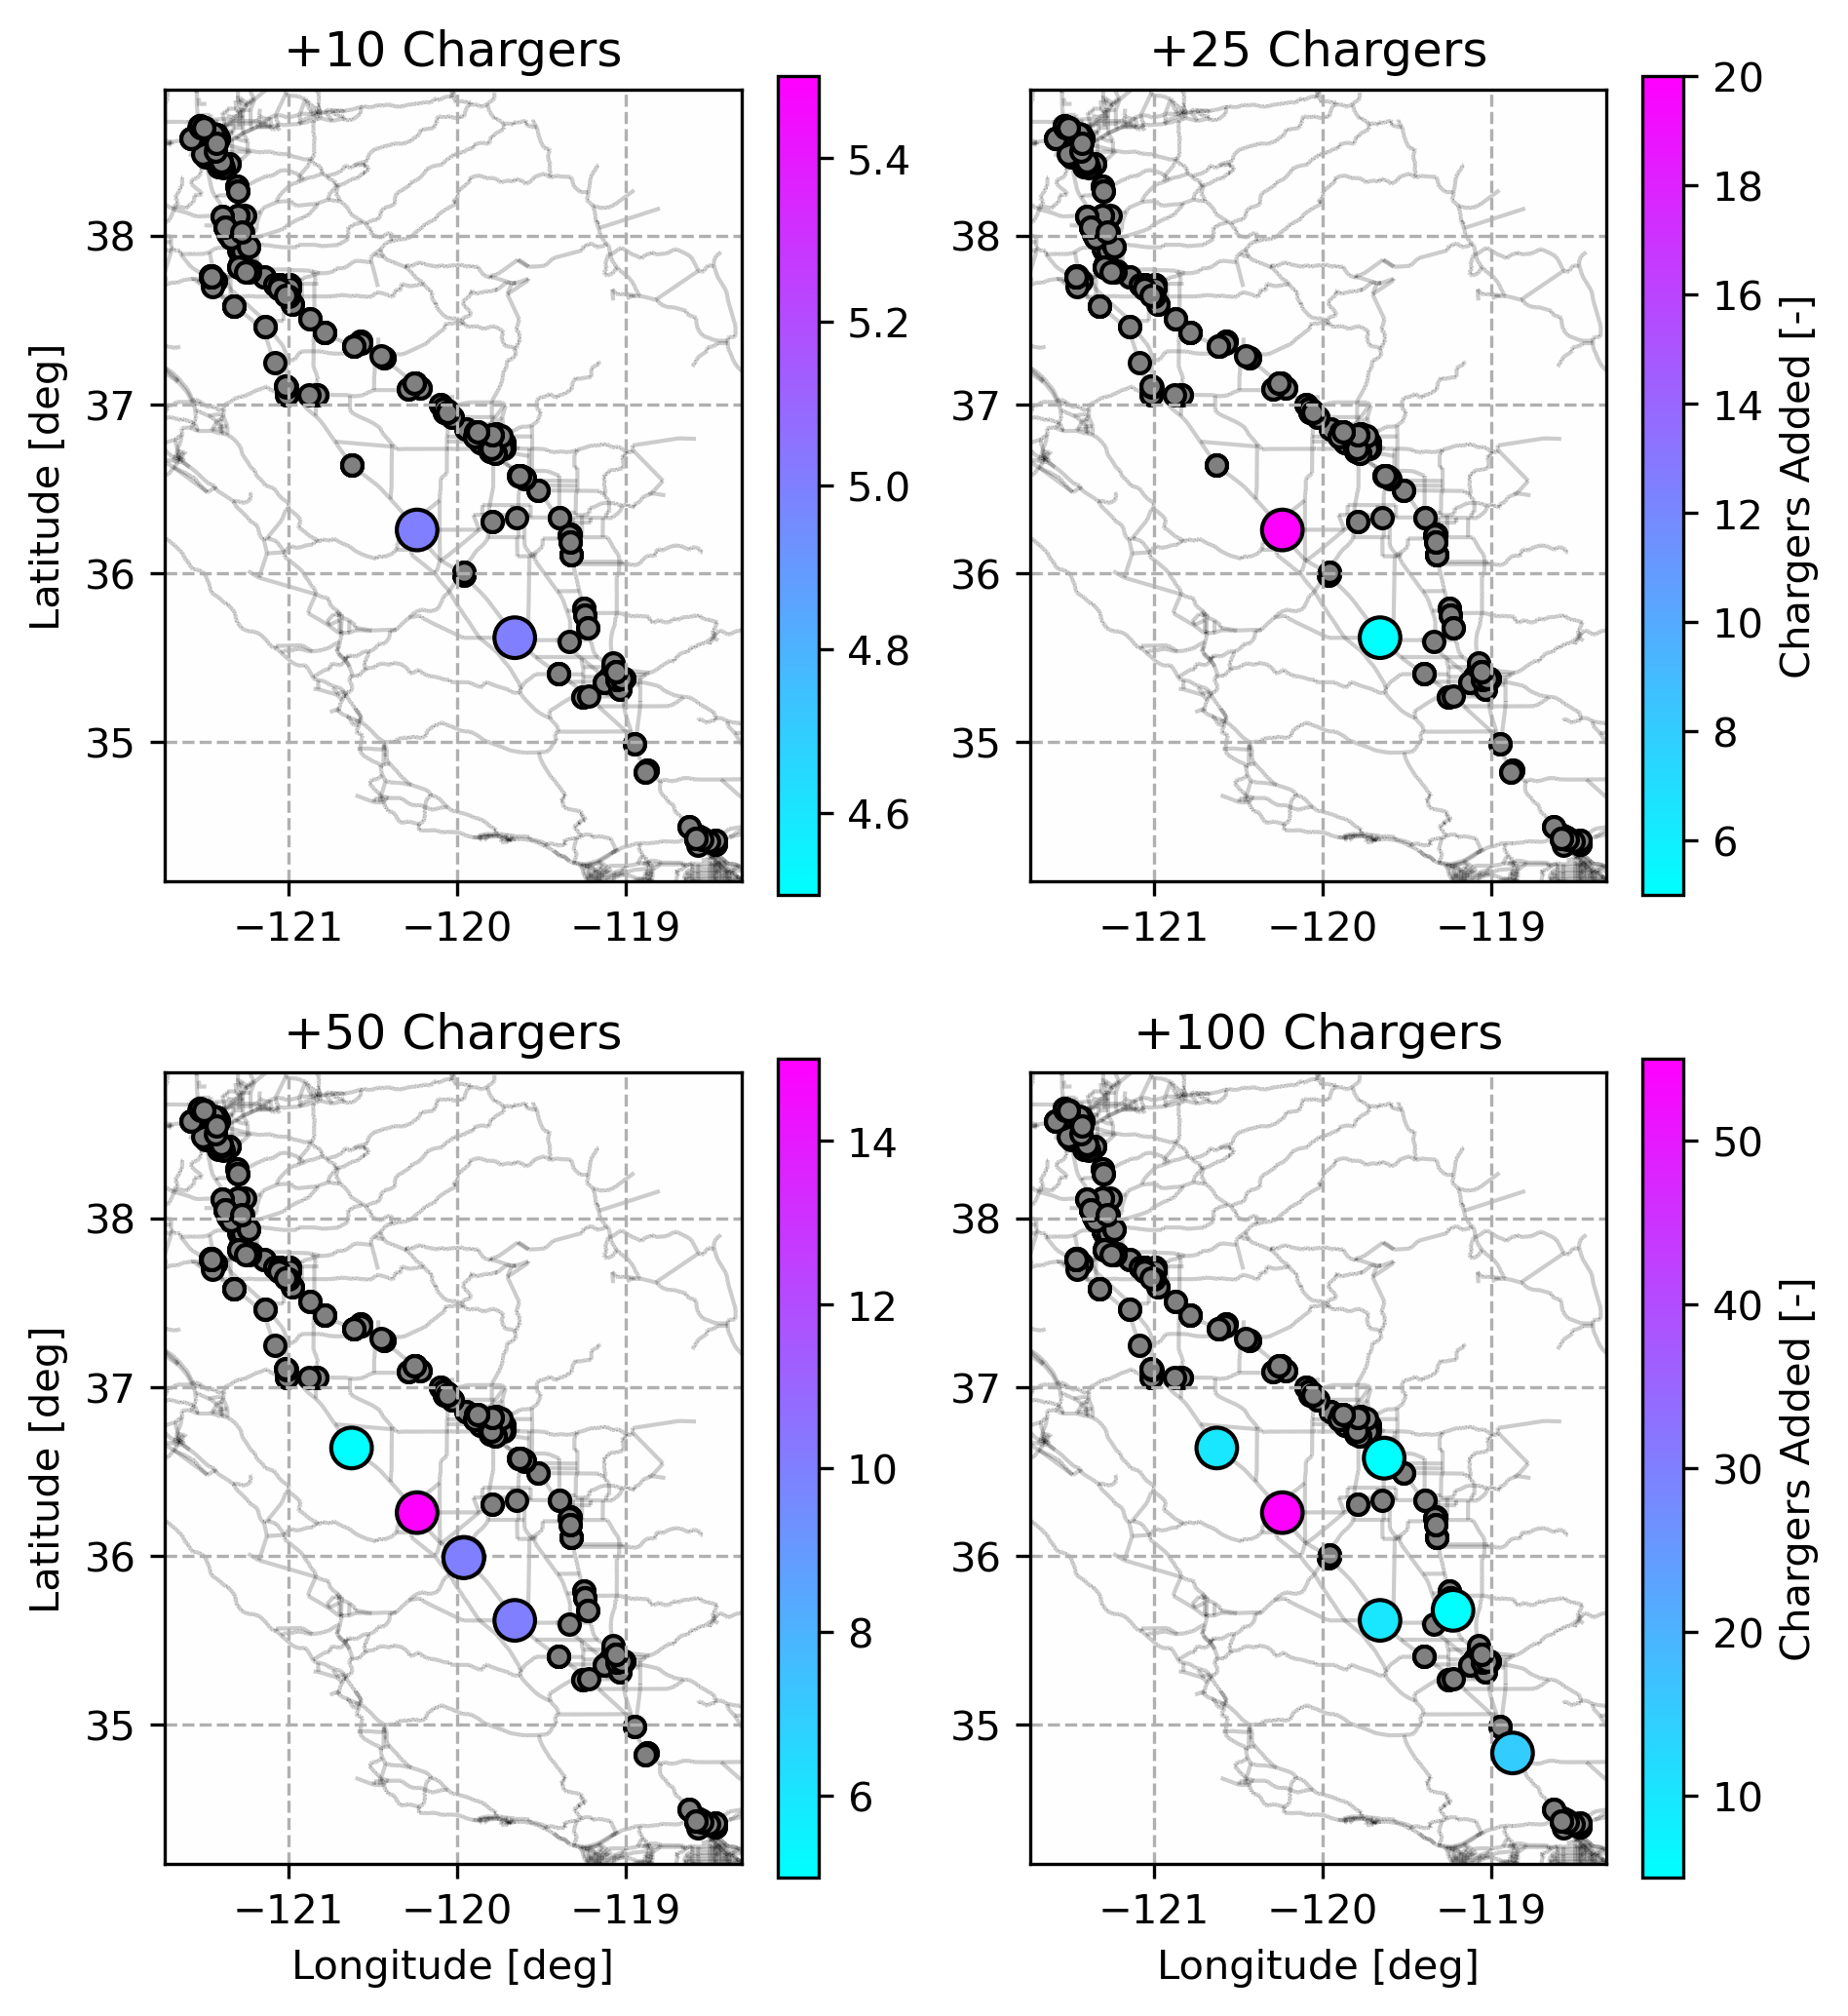
\includegraphics[width = \figurewidth]{./figures/augmented_esns.png}
	\caption{Optimal allocations of 10, 25, 50, and 100 additional chargers for CCS \gls{esn}.}
	\label{fig:augmented_esns}
\end{figure}

The optimal allocations of additional chargers broadly favor large stations on Interstate 5 and towards the center of the corridor. This is an intuitive allocation. The 5-99 corridor is of a distance where vehicles from many, but not all, cities can reach the half-way point before needing to charge. Interstate 5 is on the shortest road-path for many more origin-destination pairs than CA-99 is. Adding large stations in this area should substantially improve the corridor for travelers moving from norther California to southern California. It is not a coincidence that large Tesla stations are located in the same area. The additional chargers impact on corridor performance is shown in Figure \ref{fig:augmented_esn_performance}.

\begin{figure}[H]
	\centering
	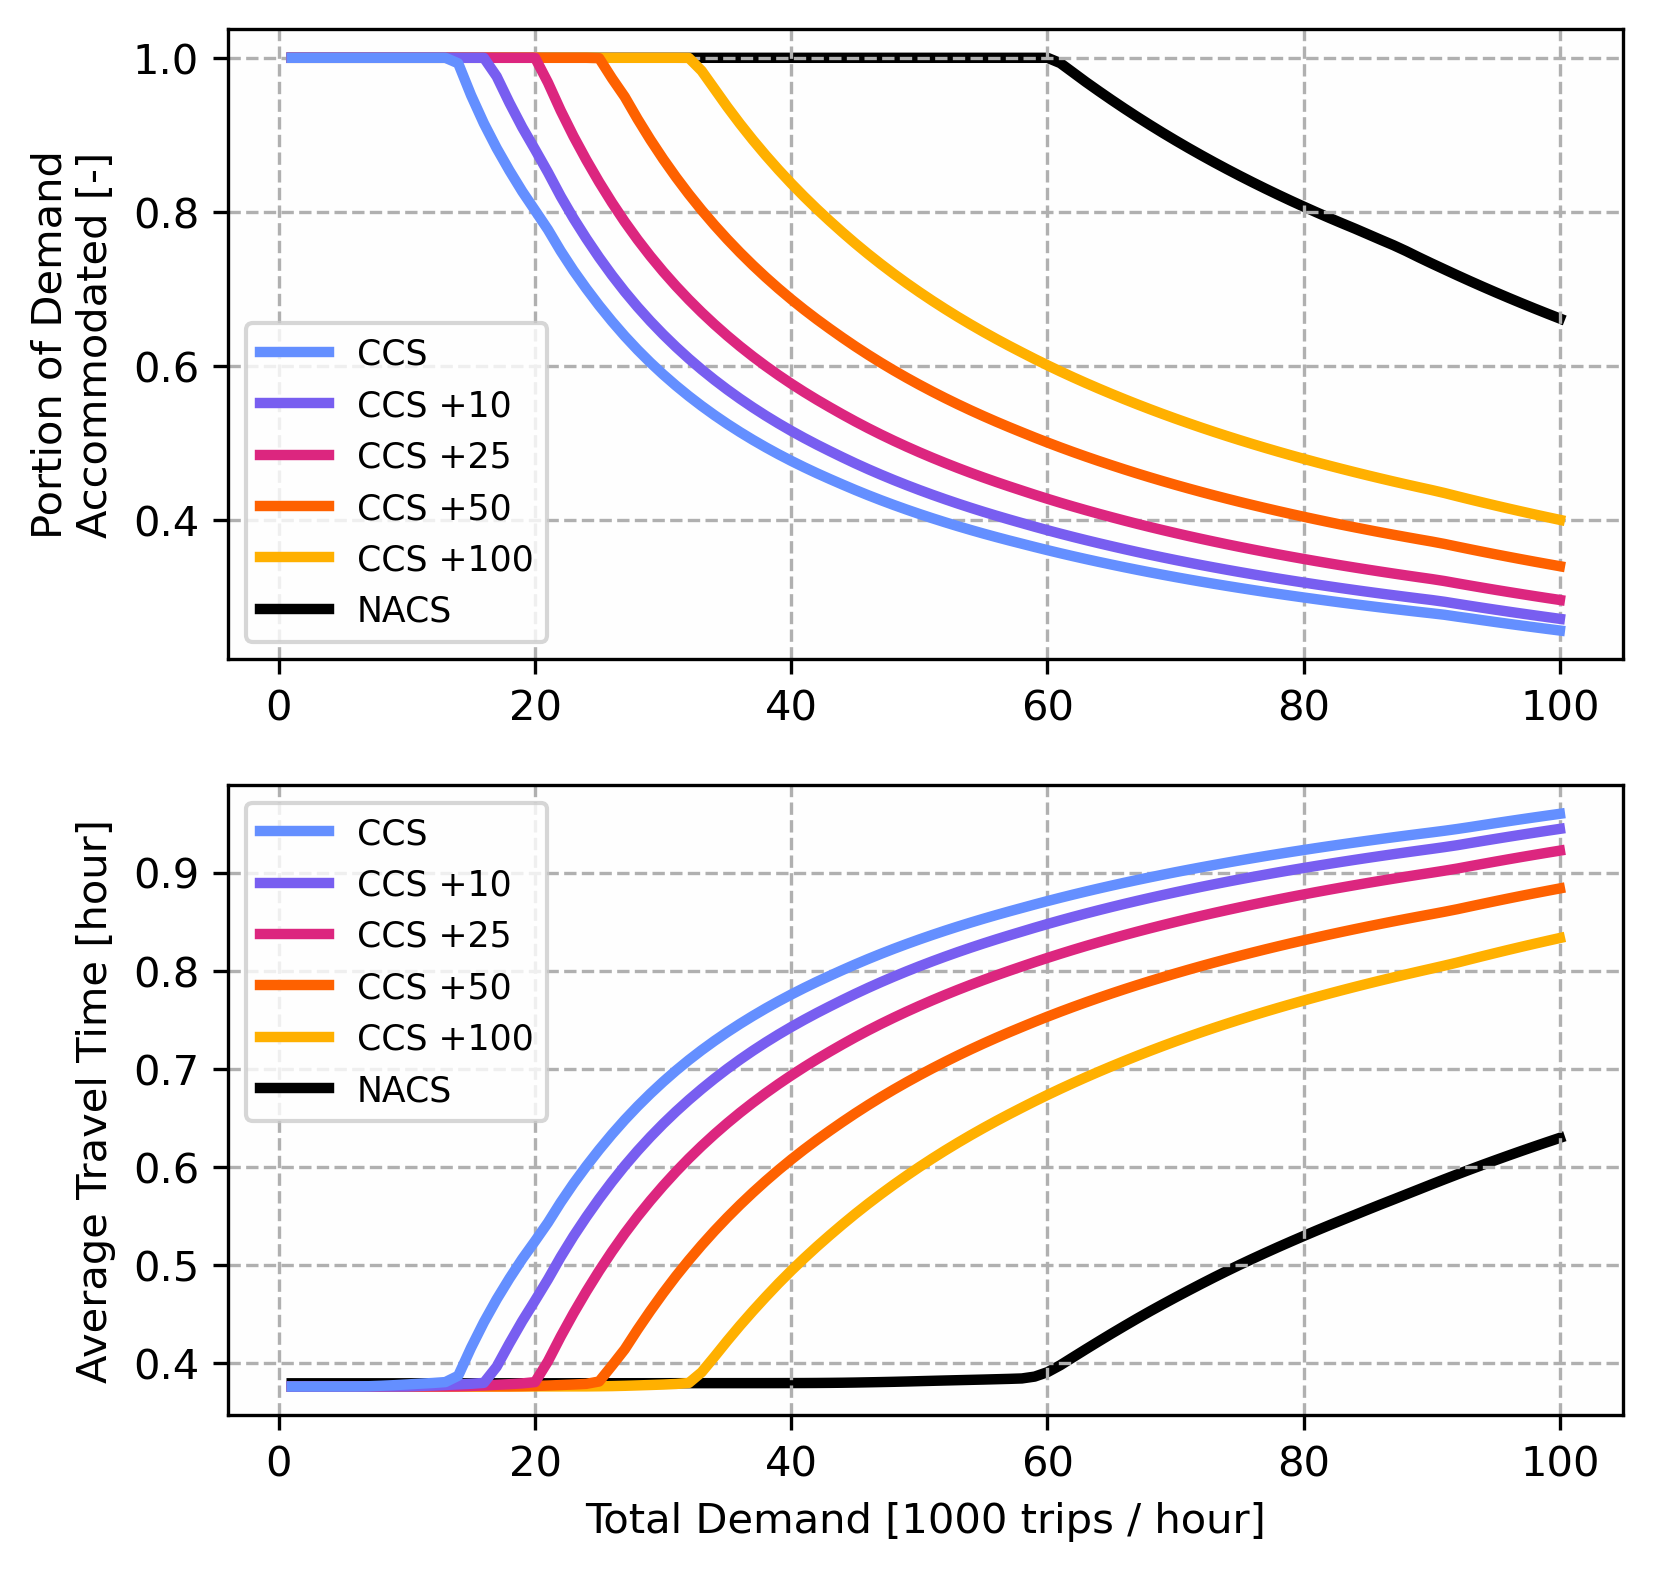
\includegraphics[width = \figurewidth]{./figures/augmented_esn_performance.png}
	\caption{Performance of NACS, CCS, and augmented CCS \glspl{esn} with increasing demand.}
	\label{fig:augmented_esn_performance}
\end{figure}

Per the optimization results, substantial improvements in \gls{esn} performance can be attained by the strategic addition of a small number of chargers if they are allocated to form large stations in high traffic locations. The large stations added along Interstate 5 offer two benefits. The first is the already discussed benefit of increased station efficiency. The second benefit is increasing the number of trips along Interstate 5 as opposed to CA-99. Interstate 5 is a more direct route and has a higher speed limit. Vehicles traveling across the 5-99 corridor on Interstate save substantial driving time. As currently configures, the CCS \gls{esn} has more capacity along CA-99 and, thus, as the number of vehicles increases a higher portion are sent along this route. With the addition of several large stations along Interstate 5, much of this traffic can take Interstate 5 instead.





\section{Conclusions}

In most senses, \glspl{bev} behave similarly or identically to \glspl{icev}. The primary advantage of \glspl{bev} in day-to-day use is the flexibility and economy afforded by charging compared to fueling. This strength becomes a drawback for long trips where slower energizing rates and less mature infrastructure impose a travel-time tax on \gls{bev} drivers substantially above that imposed on \gls{icev} drivers. Charging speeds and charging equipment costs are technical issues which may be fundamental. Much more readily addressable are the inefficient structure of the DC \gls{esn} and the policies which have guided its development.

Infrastructure networks often develop in three phases; connecting, balancing, and hardening. In the first phase minimum service is provided, in the second phase high demand elements are upgraded, and in the third phase, redundant elements are added to maintain functionality in the case of element saturation or failure. Optimal network expansion problems reduce to a simple question: how to best allocate the next batch of resources. In the connecting phase, any additional resource should be used to increase the portion of potential users that can utilize to the network. In turn, the metric of optimization is simply connectivity. In the balancing phase the metric of optimization becomes performance.

This paper introduces a novel methodology for the optimal expansion of \glspl{esn} sensitive to station congestion. This methodology represents a paradigm shift from a connectivity mindset ot a balancing mindset. This paper introduces the methodology and deploys it in a relevant and important real-life case study on a large network. The Case study, concerning the central California highway corridor DC \gls{esn} demonstrates the impact network structure on performance as demand increases. The case study also shows the utility of the methodology in generating cost-efficient improvements to existing \glspl{esn}. 
\section{Future Work}

This study introduces methodology that will be extended and applied in future work. Although possible, this study did not explicitly extend the methodology to simultaneously account for nodal and travel demand. This extension would be beneficial in order to understand how these two forms of charging demand interact with one-another and impact \gls{esn} performance. The primary limitation of the methodology is that it assumes system-level optimal routing, an altruistic behavior not likely to be seen in the real-world. Future studies will include a portion of demand whose routing is controlled by separate, non-optimal strategies in order to understand the impact that this will have on both \gls{esn} performance and optimal structure. 

\printbibliography[heading=bibintoc,title={References}]
%\bibliographystyle{ieeetr}
%\bibliography{./sources/sources}

%\end{multicols}

\end{document}